\documentclass[10pt,journal]{IEEEtran} 
\IEEEoverridecommandlockouts 
% {The preceding line is only needed to identify funding in the    first footnote. If that is unneeded, please comment it out.} 
\usepackage[utf8]{inputenc} 
\usepackage{longtable} 
\usepackage{cite}  
\usepackage{amsmath,amssymb,amsfonts} 
\usepackage{algorithmic} 
\usepackage{makeidx}
\usepackage{graphicx} 
\usepackage{textcomp} 
\usepackage{xcolor} 
\usepackage{graphicx}
\usepackage{float}
\usepackage{multicol}
\usepackage{ifpdf}
\usepackage{tikz} 
\usepackage{parskip} 
\usepackage[siunitx, american]{circuitikz}
\usetikzlibrary{automata, positioning, shapes, arrows} 
\ifpdf
\usepackage[breaklinks,hidelinks]{hyperref}
\else 
\usepackage{url}
\fi
\def\BibTeX{{\rm B\kern-.05em{\sc i\kern-.025em b}\kern-.08em 
    T\kern-.1667em\lower.7ex\hbox{E}\kern-.125emX}} 
\usepackage{parskip} 
\begin{document} 
\title{\textrm {Set Theory Foundation for the Description of \\ SR Flipflop        Digital Circuits and Signals}\\  
%{\footnotesize \textsuperscript{*}Note: Sub-titles are not captured in Xplore and should not be used} 
\thanks{\IEEEcompsocthanksitem Electronics, Instrumentation \& Control Mechatronics Engineering,              \newline Batangas State University
}} 
\author{\IEEEauthorblockN{ Engr Celso Bation Co, Ph.D, PECE,~\IEEEmembership{Member,~IEEE}} \\ 
\IEEEauthorblockA{\textit{Electronics, Instrumentation \& Control Mechatronics Engineering} \\ 
\textit{Batangas State University}\\ Batangas City, Philippines \\ 
celso.co@g.batstate-u.edu.ph} \\ \ \\ 
 }
\maketitle  
\markboth{International Research Journal on Innovations in Engineering (IRJIEST) 2021}%
    {Shell \MakeLowercase{\textit{et al.}}: Bare Advanced Demo of     IEEEtran.cls for IEEE Computer Society Journals}
\begin{abstract}The SR (Set/Reset) Flipflop was the basic component of digital logic cirtcuits. There exists certain problem in articulating the behaviour of its circuits and signals characteristics from theoretical perspective. Although the cross couple OR gate with Inverter circuit had long been established, there existed a curiosity whether it can be synthersized out of the analysis of the input and output signals of SR Flipflop Gate. The characteristics of digital signal pulses was studied with the set theory as the working paradigm. The classification of pulses was designed taking into consideration the changes of logic state in an event. The prior and post event were conceptualized that provided meaningful platform of the pulses classification. The relation and equation of set theory were instrumental in the construction of simple latch and SR flipflop circuits. The signal behaviors were shown consistent with the design equations for  prior and post events. The operation of set theory on symbolic pulses were consistent.\end{abstract}
\begin{IEEEkeywords}set theory, prior event, post event, pulse classification, SR flipflop,     simple latch, OR Gate, Inverter \end{IEEEkeywords}
\section{Preliminary}
Consider the piecewise signal as follows.
\begin{equation}
 \begin{minipage}{250pt}
\begin{flushleft} $\displaystyle \operatorname{S_{ignal}}{\left(t \right)} = \begin{cases} 0 & \\  \text{for}\: \left(t \geq 0 \wedge t < 5\right) \vee \left(t \geq 10 \wedge t < 15\right) \\ \quad \ \  \vee \left(t \geq 17 \wedge t < 23\right) \vee \left(t \geq 24 \wedge t < 34\right) \\ \quad \ \  \vee \left(t \geq 39 \wedge t < 40\right) \vee \left(t \geq 45 \wedge t < 50\right) \\ \quad \ \  \vee \left(t \geq 55 \wedge t < 57\right) \vee \left(t \geq 67 \wedge t < 75\right) \\1 & \\  \text{otherwise} \end{cases}$  \end{flushleft}
 \end{minipage}
 \end{equation}
The signal(t) could be expressed in term of set of unit time when logic     transition occurred. The transition could be either from 0 to 1 or 1 to 0.     It depended on the initial logic state. The initial logic state was      either 0 or 1 at the first item of the list. For this case, the initial     state was 0 or say stream[0]=0. Thereafter stream[5]=1, stream[10]=0,     stream[15]=1 and so on. The symbol | represened the transition edge at specified     domain unit.
\begin{equation}
 \begin{minipage}{250pt}
\begin{flushleft} $\displaystyle stream(|) = \newline  [0, 5, 10, 15, 17, 23, 24, 34, 39, 40, 45, 50, 55, 57, 67, 75, 80]$  \end{flushleft}
 \end{minipage}
 \end{equation}
The inverse of (2) looked the same as (2) except for stream[0]=1. See Figure 2 "Inverse of Stream" plot. Hence.
\begin{equation}
 \begin{minipage}{250pt}
\begin{flushleft} $\displaystyle Inverse(stream(|))  = [1, 5, 10, 15, 17, 23, 24, 34, 39, 40, 45, 50, 55, 57, 67, 75, 80]$  \end{flushleft}
 \end{minipage}
 \end{equation}
The signal(t) was plotted in Figure 1. The annotations were Top Pulses,    Top Unit, Top Impulse, Rise Pulse, Bottom Impulse, Bottom Unit Pulse,    Fall Pulse, and Bottom Pulses.    \\ \ \\    The stem plot of Figure 1 is shown in Figure 2 with the same annotations. 
\begin{figure}[H]
\centering\includegraphics[width=1\linewidth,height=0.15\textheight]{FG001.png}
\caption{Classification of Pulses}
\label{fig:FG001.png}
\end{figure}

\begin{figure}[H]
\centering\includegraphics[width=1\linewidth,height=0.15\textheight]{FG002.png}
\caption{Inverse and Stem Plot of Figure 1}
\label{fig:FG002.png}
\end{figure}

\subsection{Definition}
The logic level at a given point in time is either low (.) or high    ($\vert$) called stem. The event was represented by a couple of points in     time and defined in Table 1.
\begin{table}[H] \caption{Event Classification}\centering\begin{tabular}{|p{.4cm}|p{2cm}|p{1cm}|p{1cm}|p{1.5cm}|}\hline Item&Event Description &Stem Symbol&Stem Values &Remarks\\ \hline 00& low      &$..$ &[0,0] &no change\\ \hline 01& rise     &$.|$ &[0,1] &change\\ \hline 02& fall     &$|.$ &[1,0] &change\\ \hline 03& high     &$||$ &[1,1] &no change\\ \hline \end{tabular} \end{table} 
Let a tuple of 3 units of time be defined as follows.     Tri-unit = \{prior, current, post\} = \{t-1, t, t+1\} = t where the t     could be used as the name of the set, e.g. 25 = \{24,25,26 \}. The anchor     was t=25. The prior event of tri-unit was prior = \{t-1, t\}=\{24,25\} while     the post event of it was post = \{t,t+1\}=\{25,26\}. The pulse clasification     and their symbols were shown in Table II.
\begin{table}[H] \caption{Symbolic Pulses Classification}\centering\begin{tabular}{|p{.4cm}|p{1.6cm}|p{.9cm}|p{.9cm}|p{.8cm}|p{.5cm}|p{.5cm}|}\hline Item&Pulse Description &Pulse Symbol&Stem Symbol&Stem Values                        &Prior Event&Post Event            \\   \hline 00& bottom       &$\sqcup$ &$...$ &[0,0,0]                          &$..$ &$..$ \\ \hline 01& delay rise   &$.\nearrow$ &$..|$ &[0,0,1]                          &$..$ &$.|$ \\ \hline 02& fall         &$\searrow$ &$|..$ &[1,0,0]                          &$|.$ &$..$\\ \hline 03& impulse (-)  &$\top$ &$|.|$ &[1,0,1]                          &$|.$ &$.|$\\ \hline 04& impulse (+)  &$\bot$ &$.|.$ &[0,1,0]                          &$.|$ &$|.$\\ \hline 05& rise         &$\nearrow$ &$.||$ &[0,1,1]                          &$.|$ &$||$\\ \hline 06& delay fall   &$^.\searrow$ &$||.$ &[1,1,0]                          &$||$ &$|.$\\ \hline 07& top          &$\sqcap$ &$|||$ &[1,1,1]                          &$||$ &$||$\\ \hline \end{tabular} \end{table} 
Let following functions be defined.
\begin{equation}
 \begin{minipage}{250pt}
\begin{flushleft} $\displaystyle \operatorname{P_{rior}}{\left(P_{ulse} \right)} = \left( t - 1, \  t\right)$  \end{flushleft}
 \end{minipage}
 \end{equation}
\begin{equation}
 \begin{minipage}{250pt}
\begin{flushleft} $\displaystyle \operatorname{P_{ost}}{\left(P_{ulse} \right)} = \left( t, \  t + 1\right)$  \end{flushleft}
 \end{minipage}
 \end{equation}
\begin{equation}
 \begin{minipage}{250pt}
\begin{flushleft} $\displaystyle \operatorname{P_{ulse}}{\left(P_{ulse} \right)} = \left( t - 1, \  t, \  t + 1\right)$  \end{flushleft}
 \end{minipage}
 \end{equation}
\begin{equation}
 \begin{minipage}{250pt}
\begin{flushleft} $\displaystyle \operatorname{P_{ulse}}{\left(P_{ulse} \right)} = \operatorname{P_{ost}}{\left(P_{ulse} \right)}  \cup  \operatorname{P_{rior}}{\left(P_{ulse} \right)} = \left( t - 1, \  t, \  t  \cup  1\right)$  \end{flushleft}
 \end{minipage}
 \end{equation}
For example,$\operatorname{P_{rior}}{\left(\nearrow \right)} = .|$ and $\operatorname{P_{ost}}{\left(\nearrow \right)} = ||$ and $\operatorname{P_{ulse}}{\left(\nearrow \right)} = .||$, the anchor is the common element t. \\ \ \\     The inverse function was the compliment of the signal and the overline     represent the inverse made.
\begin{equation}
 \begin{minipage}{250pt}
\begin{flushleft} $\displaystyle \sqcup = \operatorname{I_{nv}}{\left(\sqcap \right)} = \overline\sqcap$  \end{flushleft}
 \end{minipage}
 \end{equation}
\begin{equation}
 \begin{minipage}{250pt}
\begin{flushleft} $\displaystyle \bot = \operatorname{I_{nv}}{\left(\top \right)} = \overline\top$  \end{flushleft}
 \end{minipage}
 \end{equation}
The definition of pulses in terms of tri-unit of time ensured that the     logic state change occurred during the prior event. When there was no    change in prior event but a change occurred in post event, the pulse     was said to be delayed. The presence of the dot before the symbol indicated     the delay.\\ \ \\ 
The top unit pulse was a sequence of the rise event followed by fall event.     It was a sequence of pulses, [$\nearrow$,$^.\searrow$. 
\begin{equation}
 \begin{minipage}{250pt}
\begin{flushleft} $\displaystyle \nearrow\searrow = \left( 0, \  1, \  1, \  0\right) = \left( \nearrow, \  ^.\searrow\right)$  \end{flushleft}
 \end{minipage}
 \end{equation}
In like manner bottom unit pulse,
\begin{equation}
 \begin{minipage}{250pt}
\begin{flushleft} $\displaystyle \operatorname{I_{nv}}{\left(\nearrow\searrow \right)} = \left( 1, \  0, \  0, \  1\right) = \left( \searrow, \  .\nearrow\right)$  \end{flushleft}
 \end{minipage}
 \end{equation}
The positive impulse was an intersection of rise pulse $\nearrow$ and delayed fall $^.\searrow$.
\begin{equation}
 \begin{minipage}{250pt}
\begin{flushleft} $\displaystyle \bot = \nearrow \cap ^.\searrow$  \end{flushleft}
 \end{minipage}
 \end{equation}
The negative impulse was a union of $\searrow$ and $.\nearrow$.
\begin{equation}
 \begin{minipage}{250pt}
\begin{flushleft} $\displaystyle \top = \searrow \cup .\nearrow$  \end{flushleft}
 \end{minipage}
 \end{equation}
The transition pulses were changes in logic state either 0 to 1 or 1 to 0     at prior event. The change at post event without change at prior event was     a delayed transition.
\begin{equation}
 \begin{minipage}{250pt}
\begin{flushleft} $\displaystyle | = (\nearrow, \searrow, \bot,\top)$  \end{flushleft}
 \end{minipage}
 \end{equation}
The plots for the eigth categories of pulses were illustrated in Figure 3.
\begin{figure}[H]
\centering\includegraphics[width=1\linewidth,height=0.35\textheight]{FG003.png}
\caption{Type of Pulses Categorized by the Logic State of the Left and Right Adjacent Unit of time}
\label{fig:FG003.png}
\end{figure}

\subsection{Expression}
The pulse symbol could be an expression of function. The list of pulses     in a signal was expressed as follows.
\begin{equation}
 \begin{minipage}{250pt}
\begin{flushleft} $\displaystyle \operatorname{P_{ulse}}{\left(Signal \right)} = [t_{a},t_{b},t_{c},... ,t_{n-1},t_{n},t_{n+1},    t_{k}, ...]$  \end{flushleft}
 \end{minipage}
 \end{equation}
where $t_{n-1}=1,t_{n}=1,t_{n+1}=1$ \\ \ \\ For example,
\begin{equation}
 \begin{minipage}{250pt}
\begin{flushleft} $\displaystyle \sqcap{\left(Signal \right)} = [6, 7, 8, 35, 36, 37, 41, 42, 43, 51, 52, 53, 58, 59, \newline  60, 61, 62, 63, 64, 65, 76, 77, 78]$  \end{flushleft}
 \end{minipage}
 \end{equation}
For t=35 from (16), 
\begin{equation}
 \begin{minipage}{250pt}
\begin{flushleft} $\displaystyle \sqcap{\left(Signal \right)}[35] = (Signal[34], Signal[35], Signal[36]) = (1,1,1)$  \end{flushleft}
 \end{minipage}
 \end{equation}
Another example,
\begin{equation}
 \begin{minipage}{250pt}
\begin{flushleft} $\displaystyle \uparrow{\left(Signal \right)}[34] = (Signal[33], Signal[34], Signal[35]) = (0,1,1)$  \end{flushleft}
 \end{minipage}
 \end{equation}
The union of (17) and (18), 
\begin{equation}
 \begin{minipage}{250pt}
\begin{flushleft} $\displaystyle \sqcap{\left(\operatorname{S_{ignal}}{\left(35 \right)} \right)}  \cup  \uparrow{\left(\operatorname{S_{ignal}}{\left(34 \right)} \right)} = \left\{\nearrow, \sqcap\right\}$  \end{flushleft}
 \end{minipage}
 \end{equation}
A signal could be expressed as list of symbolic pulses. Hence, given \\ 
A = \begin{tabular}{p{6cm}}      [0,  \#  A[ 0]=undefined\\       \ 0,  \#  A[ 1]=$\sqcup$\\       \ 0,  \#  A[ 2]=$.\nearrow$\\       \ 1,  \#  A[ 3]=$\nearrow$\\       \ 1,  \#  A[ 4]=$\sqcap$\\       \ 1,  \#  A[ 5]=$^.\searrow$\\       \ 0,  \#  A[ 6]=$\searrow$\\       \ 0,  \#  A[ 7]=$\sqcup$\\       \ 0,  \#  A[ 8]=$.\nearrow$\\       \ 1,  \#  A[ 9]=$\bot$\\       \ 0,  \#  A[10]=$\searrow$\\       \ 0,  \#  A[11]=$\sqcup$\\       \ 0,  \#  A[12]=$.\nearrow$\\       \ 1,  \#  A[13]=$\nearrow$\\       \ 1,  \#  A[14]=$^.\searrow$\\       \ 0,  \#  A[15]=$\top$\\       \ 1,  \#  A[16]=$\nearrow$\\       \ 1,  \#  A[17]=$^.\searrow$\\       \ 0,  \#  A[18]=$\searrow$\\       \ 0,  \#  A[19]=$.\nearrow$\\       \ 1,  \#  A[20]=$\nearrow$\\       \ 1,  \#  A[21]=$^.\searrow$\\       \ 0,  \#  A[22]=$\searrow$\\       \ 0,  \#  A[23]=$\sqcup$\\       \ 0   \#  A[24]=undefine ]        \end{tabular} \\ \ \\ 
The sequence of pulses in A were [$\sqcup$, $.\nearrow$, $\nearrow$, $\sqcap$, $^.\searrow$, $\searrow$, $\sqcup$, $.\nearrow$, $\bot$, $\searrow$, $\sqcup$, $.\nearrow$, $\nearrow$, $^.\searrow$, $\top$, $\nearrow$, $^.\searrow$, $\searrow$, $.\nearrow$, $\nearrow$, $^.\searrow$, $\searrow$, $\sqcup$]   
\section{Signal Sets}
Let's examine the of signal sets behavior in both open and closed systems     logic circuit. The open loop system was a feed forward and without a feedback.     The closed system has feedback loop.
\subsection{Combinatory Logic: Open Loop System}
A given set of signals had a combinations of a number of pulses, impulses,    rising and falling edges and their inverses. It could also be said that any    signal was a set of time points of stems. A stem represented an impulse.    Two consecutive stems represent a rising and a falling pulse. Three    consecutive stems makes a pulse. A stem was identified by its location in    time domain. A point in time could be classified as a pulse, a rising edge,    a falling edge, an impulse and their inverses depending on the changes of its    prior and post events. A stem was defined as logic state 1 at a point    in time domain.\\ \ \\    Consider the followins signals 
\begin{equation}
 \begin{minipage}{250pt}
\begin{flushleft} $\displaystyle A{\left(t \right)} = \begin{cases} 0 & \\  \text{for}\: \left(t \geq 0 \wedge t < 4\right) \vee \left(t \geq 8 \wedge t < 11\right) \\ \quad \ \  \vee \left(t \geq 12 \wedge t < 15\right) \vee \left(t \geq 20 \wedge t < 22\right) \\ \quad \ \  \vee \left(t \geq 23 \wedge t < 31\right) \vee \left(t \geq 34 \wedge t < 38\right) \\ \quad \ \  \vee \left(t \geq 48 \wedge t < 50\right) \\1 & \\  \text{otherwise} \end{cases}$  \end{flushleft}
 \end{minipage}
 \end{equation}
\begin{table}[H] \caption{Signal A Pulses}\centering\begin{tabular}{|p{.4cm}|p{.5cm}|p{6.5cm}|}\hline Item&Pulse &Stem Set\\ \hline 00& \footnotesize$\sqcap$ & \footnotesize[5, 6, 16, 17, 18, 32, 39, 40, 41, 42, 43, 44, 45, 46]\\ \hline 01& \footnotesize$\sqcup$ & \footnotesize[1, 2, 9, 13, 24, 25, 26, 27, 28, 29, 35, 36]\\ \hline 02& \footnotesize$\nearrow$ & \footnotesize[4, 15, 31, 38]\\ \hline 03& \footnotesize$\searrow$ & \footnotesize[8, 12, 20, 23, 34, 48]\\ \hline 04& \footnotesize$\bot$ & \footnotesize[11, 22]\\ \hline 05& \footnotesize$\top$ & \footnotesize[]\\ \hline 06& \footnotesize$.\nearrow$ & \footnotesize[3, 10, 14, 21, 30, 37]\\ \hline 07& \footnotesize$^.\searrow$ & \footnotesize[7, 19, 33, 47]\\ \hline 08& \footnotesize$|$ & \footnotesize[4, 8, 11, 12, 15, 20, 22, 23, 31, 34, 38, 48]\\ \hline \end{tabular} \end{table} 
\begin{equation}
 \begin{minipage}{250pt}
\begin{flushleft} $\displaystyle B{\left(t \right)} = \begin{cases} 1 & \\  \text{for}\: \left(t \geq 0 \wedge t < 2\right) \vee \left(t \geq 7 \wedge t < 9\right) \vee \left(t \geq 18 \wedge t < 25\right) \\ \quad \ \  \vee \left(t \geq 26 \wedge t < 28\right) \vee \left(t \geq 30 \wedge t < 36\right) \\ \quad \ \  \vee \left(t \geq 40 \wedge t < 42\right) \vee \left(t \geq 43 \wedge t < 46\right) \\0 & \\  \text{otherwise} \end{cases}$  \end{flushleft}
 \end{minipage}
 \end{equation}
\begin{table}[H] \caption{Signal B Pulses}\centering\begin{tabular}{|p{.4cm}|p{.5cm}|p{6.5cm}|}\hline Item&Pulse &Stem Set\\ \hline 00& \footnotesize$\sqcap$ & \footnotesize[19, 20, 21, 22, 23, 31, 32, 33, 34, 44]\\ \hline 01& \footnotesize$\sqcup$ & \footnotesize[3, 4, 5, 10, 11, 12, 13, 14, 15, 16, 37, 38, 47, 48]\\ \hline 02& \footnotesize$\nearrow$ & \footnotesize[7, 18, 26, 30, 40, 43]\\ \hline 03& \footnotesize$\searrow$ & \footnotesize[2, 9, 28, 36, 46]\\ \hline 04& \footnotesize$\bot$ & \footnotesize[]\\ \hline 05& \footnotesize$\top$ & \footnotesize[25, 42]\\ \hline 06& \footnotesize$.\nearrow$ & \footnotesize[6, 17, 29, 39]\\ \hline 07& \footnotesize$^.\searrow$ & \footnotesize[1, 8, 24, 27, 35, 41, 45]\\ \hline 08& \footnotesize$|$ & \footnotesize[2, 7, 9, 18, 25, 26, 28, 30, 36, 40, 42, 43, 46]\\ \hline \end{tabular} \end{table} 
\begin{table}[H] \caption{Signal C = A $\cup$ B Pulses}\centering\begin{tabular}{|p{.4cm}|p{.5cm}|p{6.5cm}|}\hline Item&Pulse &Stem Set\\ \hline 00& \footnotesize$\sqcap$ & \footnotesize[5, 6, 7, 16, 17, 18, 19, 20, 21, 22, 23, 31, 32, 33, 34, 39, 40, 41, 42, 43, 44, 45, 46, 51, 52, 53]\\ \hline 01& \footnotesize$\sqcup$ & \footnotesize[13]\\ \hline 02& \footnotesize$\nearrow$ & \footnotesize[4, 15, 26, 30, 38, 50]\\ \hline 03& \footnotesize$\searrow$ & \footnotesize[2, 9, 12, 28, 36, 48]\\ \hline 04& \footnotesize$\bot$ & \footnotesize[11]\\ \hline 05& \footnotesize$\top$ & \footnotesize[25]\\ \hline 06& \footnotesize$.\nearrow$ & \footnotesize[3, 10, 14, 29, 37, 49]\\ \hline 07& \footnotesize$^.\searrow$ & \footnotesize[1, 8, 24, 27, 35, 47]\\ \hline 08& \footnotesize$|$ & \footnotesize[2, 4, 9, 11, 12, 15, 25, 26, 28, 30, 36, 38, 48, 50]\\ \hline \end{tabular} \end{table} 
\begin{table}[H] \caption{Signal D = A $\cap$ B Pulses}\centering\begin{tabular}{|p{.4cm}|p{.5cm}|p{6.5cm}|}\hline Item&Pulse &Stem Set\\ \hline 00& \footnotesize$\sqcap$ & \footnotesize[32, 44]\\ \hline 01& \footnotesize$\sqcup$ & \footnotesize[1, 2, 3, 4, 5, 9, 10, 11, 12, 13, 14, 15, 16, 24, 25, 26, 27, 28, 29, 35, 36, 37, 38, 47, 48, 49, 50, 51, 52, 53]\\ \hline 02& \footnotesize$\nearrow$ & \footnotesize[18, 31, 40, 43]\\ \hline 03& \footnotesize$\searrow$ & \footnotesize[8, 20, 23, 34, 46]\\ \hline 04& \footnotesize$\bot$ & \footnotesize[7, 22]\\ \hline 05& \footnotesize$\top$ & \footnotesize[42]\\ \hline 06& \footnotesize$.\nearrow$ & \footnotesize[6, 17, 21, 30, 39]\\ \hline 07& \footnotesize$^.\searrow$ & \footnotesize[19, 33, 41, 45]\\ \hline 08& \footnotesize$|$ & \footnotesize[7, 8, 18, 20, 22, 23, 31, 34, 40, 42, 43, 46]\\ \hline \end{tabular} \end{table} 
\begin{figure}[H]
\centering\includegraphics[width=1\linewidth,height=0.35\textheight]{FG004.png}
\caption{Signals A and B and their Union and Intersection    Operations}
\label{fig:FG004.png}
\end{figure}

\subsection{Simple Latch: a Closed Loop System}
A closed loop system could be illustrated by a simple latch. It was a system     consisting of an input and an output. Initial, the input is at zero logic     state and the output was likewise at zero logic state. When a pulse occured,     the output latched to logic state 1 and kept it latched irrespective of     changes in logic state at the input thereafter. See Figure 5.  Given such     signals operating condition, it was desired to derive the simple latch     circuit. Its block diagram was shown in Figure 6.\\ \ \\     The input signal $In$ and the output signal $Out$ were     defined in term of piecewise equation as follows
\begin{equation}
 \begin{minipage}{250pt}
\begin{flushleft} $\displaystyle \operatorname{In}{\left(t \right)} = \begin{cases} 0 & \\  \text{for}\: \left(t \geq 0 \wedge t < 3\right) \vee \\ \ \ \quad    \left(t \geq 4 \wedge t < 7\right) \vee \\ \ \ \quad    \left(t \geq 9 \wedge t < 10\right) \\1 & \\  \text{otherwise} \end{cases}$  \end{flushleft}
 \end{minipage}
 \end{equation}
\begin{table}[H] \caption{Signal In Pulses}\centering\begin{tabular}{|p{.4cm}|p{.5cm}|p{6.5cm}|}\hline Item&Pulse &Stem Set\\ \hline 00& \footnotesize$\sqcap$ & \footnotesize[]\\ \hline 01& \footnotesize$\sqcup$ & \footnotesize[1, 5]\\ \hline 02& \footnotesize$\nearrow$ & \footnotesize[7]\\ \hline 03& \footnotesize$\searrow$ & \footnotesize[4]\\ \hline 04& \footnotesize$\bot$ & \footnotesize[3]\\ \hline 05& \footnotesize$\top$ & \footnotesize[]\\ \hline 06& \footnotesize$.\nearrow$ & \footnotesize[2, 6]\\ \hline 07& \footnotesize$^.\searrow$ & \footnotesize[8]\\ \hline 08& \footnotesize$|$ & \footnotesize[3, 4, 7]\\ \hline \end{tabular} \end{table} 
\begin{equation}
 \begin{minipage}{250pt}
\begin{flushleft} $\displaystyle \operatorname{Out}{\left(t \right)} = \begin{cases} 0 & \\  \text{for}\: t \geq 0 \wedge t < 3 \\1 & \\  \text{otherwise} \end{cases}$  \end{flushleft}
 \end{minipage}
 \end{equation}
\begin{table}[H] \caption{Signal Out Pulses}\centering\begin{tabular}{|p{.4cm}|p{.5cm}|p{6.5cm}|}\hline Item&Pulse &Stem Set\\ \hline 00& \footnotesize$\sqcap$ & \footnotesize[4, 5, 6, 7, 8, 9, 10, 11, 12, 13]\\ \hline 01& \footnotesize$\sqcup$ & \footnotesize[1]\\ \hline 02& \footnotesize$\nearrow$ & \footnotesize[3]\\ \hline 03& \footnotesize$\searrow$ & \footnotesize[]\\ \hline 04& \footnotesize$\bot$ & \footnotesize[]\\ \hline 05& \footnotesize$\top$ & \footnotesize[]\\ \hline 06& \footnotesize$.\nearrow$ & \footnotesize[2]\\ \hline 07& \footnotesize$^.\searrow$ & \footnotesize[]\\ \hline 08& \footnotesize$|$ & \footnotesize[3]\\ \hline \end{tabular} \end{table} 
\begin{figure}[H]
\centering\includegraphics[width=1\linewidth,height=0.15\textheight]{FG005.png}
\caption{Simple Latch}
\label{fig:FG005.png}
\end{figure}

\begin{figure}[H]                                                     
   \centering                                                        
	\tikzstyle{block} = [draw, fill=white, rectangle,                 
	minimum height=1cm, minimum width=2cm]                             
	\tikzstyle{input} = [coordinate]                                  
	\tikzstyle{output} = [coordinate]                                 
	\tikzstyle{pinstyle} = [pin edge={to-,thin,black}]                
	\begin{tikzpicture}[auto, node distance=2cm,>=latex']             
	\node [input, name=input] {};                                     
	\node [block, right of=input] (Latch) {$Latch$};                  
	\node [output, right of=Latch] (out) {};                          
	\draw [draw,->] (-.5,0) node {$In(t)$} (input) -- (Latch);        
	\draw [draw,->] (Latch) --  (out)  node {};                       
	\draw (4.75,0) node {$Out(t)$};                                   
    \end{tikzpicture}                                                 
\caption{Block Diagram of Simple Latch}                               
\label{fig:Figure 6}                                                  
\end{figure}
By observation of Tables VII, VIII and Figure 5, the following relationships     were noted.
\begin{equation}
 \begin{minipage}{250pt}
\begin{flushleft} $\displaystyle \operatorname{In_{\sqcap}}{\left(t \right)} \subset \operatorname{Out_{\sqcap}}{\left(t \right)}$  constant pulses\end{flushleft}
 \end{minipage}
 \end{equation}
\begin{equation}
 \begin{minipage}{250pt}
\begin{flushleft} $\displaystyle \operatorname{In_{|}}{\left(t \right)} \supset \operatorname{Out_{|}}{\left(t \right)}$  changing pulses\end{flushleft}
 \end{minipage}
 \end{equation}
The circuit could be derived from observed behavior of the relation (24). Since relation had no equivalent real world circuit,     it was necessary to determine its equivalent equation as follows.
\begin{equation}
 \begin{minipage}{250pt}
\begin{flushleft} $\displaystyle \operatorname{Out}{\left(t \right)} = \operatorname{Out}{\left(t \right)} \cup \operatorname{In}{\left(t \right)}$  \end{flushleft}
 \end{minipage}
 \end{equation}
The equation (26) was expressed in terms of set theory. The     implementation in hardware circuit of $\cup$ set operation was the     Boolean equation for OR gate. The circuit diagram was shown in Figure 7
\begin{figure}[H]                                                             
    \centering                                                                
	\tikzstyle{block} = [draw, fill=white, rectangle,                         
	minimum height=.5cm, minimum width=1cm]                                    
	\tikzstyle{input} = [coordinate]                                          
	\tikzstyle{output} = [coordinate]                                         
	\tikzstyle{pinstyle} = [pin edge={to-,thin,black}]                        
\begin{circuitikz}                                                            
\ctikzset{tripoles/american or port/input height=.5}                          
\node[input,name=P1] {$S$};                                                   
\begin{scope}                                                                 
\ctikzset{tripoles/american or port/height=1}                                 
\draw (-.5,0) node {$\operatorname{In}{\left(t \right)}$} (P1) -- (0.5,0)                      
  node[american or port, anchor=in 1] (B) {};                                  
\end{scope}                                                                   
\node[output, right of=B, node distance=1cm] (Q) {};                          
\draw (B) -- (Q) (3.5,-.4) node {$\operatorname{Out}{\left(t \right)}$};                       
\node[input, below of =B, node distance=1cm] (fb) {};                         
%\draw (B.out) |- (fb);                                                       
%\draw (fb) -| (B.in 2);                                                      
\node[input,below of = P1, name=P2, node distance=.7cm] {};                   
\draw (-.7,-.7) node {$\operatorname{Out}{\left(t \right)}$} (P2) -- (B.in 2);                 
\end{circuitikz}                                                              
\caption{OR Gate Circuit Diagram for Simple Latch Equation $\operatorname{Out}{\left(t \right)} = \operatorname{Out}{\left(t \right)} \cup \operatorname{In}{\left(t \right)}$}                                                   
\label{fig:Figure 7}                                                          
\end{figure}
Since the $\operatorname{Out}{\left(t \right)}$ at input terminal of the OR gate was the same $\operatorname{Out}{\left(t \right)}$ at its output terminal, then the two terminal must be    connected as shown in Figure 8. Let the $Out$ at the input terminal    be tag as $In_{fb}$ keeping in mind $Out = In_{fb}$. Hence,    the existing of feed back loop made this circuit closed loop system. The    subset relation ($\operatorname{In_{\sqcap}}{\left(t \right)} \subset \operatorname{Out_{\sqcap}}{\left(t \right)}$) that depicted a feedback    equation was indicative of memrory feature. In the sequence of $\operatorname{P_{ulse}}{\left(In \right)}$ pulses, the latch happened at $\operatorname{P_{ulse}}{\left(Out \right)}$ when    a change in $\operatorname{P_{ulse}}{\left(In \right)}$ occurred as shown in Figure 8.
\begin{figure}[H]                                                             
    \centering                                                                
	\tikzstyle{block} = [draw, fill=white, rectangle,                         
	minimum height=1.5cm, minimum width=3cm]                                   
	\tikzstyle{input} = [coordinate]                                          
	\tikzstyle{output} = [coordinate]                                         
	\tikzstyle{pinstyle} = [pin edge={to-,thin,black}]                        
\begin{circuitikz}                                                            
\ctikzset{tripoles/american or port/input height=.5}                          
\node[input,name=P1] {$S$};                                                   
\begin{scope}                                                                 
\ctikzset{tripoles/american or port/height=1}                                 
\draw (-.4,0) node {$In $} (P1) -- (0.5,0)                        
  node[american or port, scale=.75, anchor=in 1] (B) {};                       
\end{scope}                                                                   
\node[output, right of=B, node distance=.5cm] (Q) {};                         
\draw (B.out) -- (Q);                                                         
\draw (2.4cm,-.3cm) node {$Out $};                                
\node [input, below of =B, node distance=1cm] (fb) {};                        
\draw (B.out) |- (fb);                                                        
\draw  (fb) -| (B.in 2);                                                      
\node[input,below of = P1, name=P2, node distance=.53cm] {};                  
\draw (-.4cm,-.55cm) node {$In_{fb}$} (P2) -- (B.in 2);             
\end{circuitikz}                                                              
\caption{OR Gate Circuit for Simple Latch Equation ($\operatorname{In_{\sqcap}}{\left(t \right)} \subset \operatorname{Out_{\sqcap}}{\left(t \right)}$)}  
\label{fig:Figure 8}                                                          
\end{figure}
Note that $\sqcup\subset\sqcup$,    $\bot\subset\nearrow$,    $\sqcup\subset\sqcap$.   The events of $In$, $In_{fb}$, and $Out$ were tabulated in    IX. The operating equations were tabulated in Table X. There were a sequence    of eigth pulses in the events. For each event, there were a set of five    equations. The first was the initial prior event condition of $In_{fb}$.     the second equation was the prior event. The third equation was the    setting of the initial post condition of $In_{fb}$. This was the    feedback action. The fourth equation was the initial post event condition of    $In_{fb}$. The fifth equation is the whole event equation.
\begin{table}[H] \caption{Simple Latch Event}\centering\begin{tabular}{|p{.3cm}|p{.6cm}|p{6.424cm}|}\hline Item&Signals &Stems \\ \end{tabular} \\ \begin{tabular}{|p{.3cm}|p{.6cm}|p{.25cm}|p{.25cm}|p{.25cm}|p{.25cm}|p{.25cm}                                 |p{.25cm}|p{.25cm}|p{.25cm}|p{.25cm}|p{.25cm}|}\hline 00&$In$&0&0&0&1&0&0&1&1&1&0 \\ \hline 01&Pulses& &$\sqcup$&$.\nearrow$&$\bot$&$\searrow$&$.\nearrow$&$\nearrow$&$\sqcap$&$^.\searrow$& \\ \hline 02&Priors& &$..$&$..$&$.|$&$|.$&$..$&$.|$&$||$&$||$& \\ \hline 03&Now   & &$...$&$..|$&$.|.$&$|..$&$..|$&$|||$&$|||$&$||.$& \\ \hline 04&Posts& &$..$&$.|$&$|.$&$..$&$.|$&$.|$&$||$&$|.$& \\ \hline 05&$In_{fb}$&0&0&0&0&1&1&1&1&1&1 \\ \hline 06&Pulses& &$\sqcup$&$\sqcup$&$.\nearrow$&$\nearrow$&$\sqcap$&$\sqcap$&$\sqcap$&$\sqcap$& \\ \hline 07&Priors& &$..$&$..$&$..$&$.|$&$||$&$||$&$||$&$||$& \\ \hline 08&Now   & &$...$&$...$&$..|$&$.||$&$|||$&$|||$&$|||$&$|||$& \\ \hline 09&Posts& &$..$&$..$&$.|$&$||$&$||$&$||$&$||$&$||$& \\ \hline 10&$Out$&0&0&0&1&1&1&1&1&1&1 \\ \hline 11&Pulses& &$\sqcup$&$.\nearrow$&$\nearrow$&$\sqcap$&$\sqcap$&$\sqcap$&$\sqcap$&$\sqcap$& \\ \hline 12&Priors& &$..$&$..$&$.|$&$||$&$||$&$||$&$||$&$||$& \\ \hline 13&Now   & &$...$&$..|$&$.||$&$|||$&$|||$&$|||$&$|||$&$|||$& \\ \hline 14&Posts& &$..$&$.|$&$||$&$||$&$||$&$||$&$||$&$||$& \\ \hline \end{tabular} \end{table} 
\begin{table}[H] \caption{Simple Latch Equation Event}\centering\begin{tabular}{|p{.05cm}|p{6.22cm}|p{1.4cm}|}\hline n&Equations & Stems \\ \hline  1  &\scriptsize $\operatorname{P_{rior}}{\left(\operatorname{In_{fb}}{\left(\sqcup \right)} \right)}$ = $\operatorname{P_{ost}}{\left(\operatorname{In_{fb}}{\left(\sqcup \right)} \right)}$&\scriptsize $..$ = $..$\\             &\scriptsize $\operatorname{P_{rior}}{\left(\operatorname{In}{\left(\sqcup \right)} \right)}$ $\cup$ $\operatorname{P_{rior}}{\left(\operatorname{In_{fb}}{\left(\sqcup \right)} \right)}$ = $\operatorname{P_{rior}}{\left(\operatorname{Out}{\left(\sqcup \right)} \right)}$&\scriptsize $..$ $\cup$ $..$ = $..$ \\             &\scriptsize  $\operatorname{P_{ost}}{\left(\operatorname{In_{fb}}{\left(\sqcup \right)} \right)}$ = $\operatorname{P_{rior}}{\left(\operatorname{Out}{\left(\sqcup \right)} \right)}$&\scriptsize  $..$ = $..$ \\             &\scriptsize  $\operatorname{P_{ost}}{\left(\operatorname{In}{\left(\sqcup \right)} \right)}$ $\cup$ $\operatorname{P_{ost}}{\left(\operatorname{In_{fb}}{\left(\sqcup \right)} \right)}$ = $\operatorname{P_{ost}}{\left(\operatorname{Out}{\left(\sqcup \right)} \right)}$&\scriptsize  $..$ $\cup$ $..$ = $..$ \\             &\scriptsize  $\operatorname{In}{\left(\sqcup \right)}$ $\cup$ $\operatorname{In_{fb}}{\left(\sqcup \right)}$ = $\operatorname{Out}{\left(\sqcup \right)}$&\scriptsize  $...$ $\cup$ $...$ = $...$ \\ \hline  2  &\scriptsize $\operatorname{P_{rior}}{\left(\operatorname{In_{fb}}{\left(\sqcup \right)} \right)}$ = $\operatorname{P_{ost}}{\left(\operatorname{In_{fb}}{\left(\sqcup \right)} \right)}$&\scriptsize $..$ = $..$\\             &\scriptsize $\operatorname{P_{rior}}{\left(\operatorname{In}{\left(.\nearrow \right)} \right)}$ $\cup$ $\operatorname{P_{rior}}{\left(\operatorname{In_{fb}}{\left(\sqcup \right)} \right)}$ = $\operatorname{P_{rior}}{\left(\operatorname{Out}{\left(.\nearrow \right)} \right)}$&\scriptsize $..$ $\cup$ $..$ = $..$ \\             &\scriptsize  $\operatorname{P_{ost}}{\left(\operatorname{In_{fb}}{\left(\sqcup \right)} \right)}$ = $\operatorname{P_{rior}}{\left(\operatorname{Out}{\left(\sqcup \right)} \right)}$&\scriptsize  $..$ = $..$ \\             &\scriptsize  $\operatorname{P_{ost}}{\left(\operatorname{In}{\left(.\nearrow \right)} \right)}$ $\cup$ $\operatorname{P_{ost}}{\left(\operatorname{In_{fb}}{\left(\sqcup \right)} \right)}$ = $\operatorname{P_{ost}}{\left(\operatorname{Out}{\left(.\nearrow \right)} \right)}$&\scriptsize  $.|$ $\cup$ $..$ = $.|$ \\             &\scriptsize  $\operatorname{In}{\left(.\nearrow \right)}$ $\cup$ $\operatorname{In_{fb}}{\left(\sqcup \right)}$ = $\operatorname{Out}{\left(.\nearrow \right)}$&\scriptsize  $..|$ $\cup$ $...$ = $..|$ \\ \hline  3  &\scriptsize $\operatorname{P_{rior}}{\left(\operatorname{In_{fb}}{\left(\sqcup \right)} \right)}$ = $\operatorname{P_{ost}}{\left(\operatorname{In_{fb}}{\left(\sqcup \right)} \right)}$&\scriptsize $..$ = $..$\\             &\scriptsize $\operatorname{P_{rior}}{\left(\operatorname{In}{\left(\bot \right)} \right)}$ $\cup$ $\operatorname{P_{rior}}{\left(\operatorname{In_{fb}}{\left(\sqcup \right)} \right)}$ = $\operatorname{P_{rior}}{\left(\operatorname{Out}{\left(\bot \right)} \right)}$&\scriptsize $.|$ $\cup$ $..$ = $.|$ \\             &\scriptsize  $\operatorname{P_{ost}}{\left(\operatorname{In_{fb}}{\left(.\nearrow \right)} \right)}$ = $\operatorname{P_{rior}}{\left(\operatorname{Out}{\left(\bot \right)} \right)}$&\scriptsize  $.|$ = $.|$ \\             &\scriptsize  $\operatorname{P_{ost}}{\left(\operatorname{In}{\left(\bot \right)} \right)}$ $\cup$ $\operatorname{P_{ost}}{\left(\operatorname{In_{fb}}{\left(.\nearrow \right)} \right)}$ = $\operatorname{P_{ost}}{\left(\operatorname{Out}{\left(\nearrow \right)} \right)}$&\scriptsize  $|.$ $\cup$ $.|$ = $||$ \\             &\scriptsize  $\operatorname{In}{\left(\bot \right)}$ $\cup$ $\operatorname{In_{fb}}{\left(.\nearrow \right)}$ = $\operatorname{Out}{\left(\nearrow \right)}$&\scriptsize  $.|.$ $\cup$ $..|$ = $.||$ \\ \hline  4  &\scriptsize $\operatorname{P_{rior}}{\left(\operatorname{In_{fb}}{\left(\nearrow \right)} \right)}$ = $\operatorname{P_{ost}}{\left(\operatorname{In_{fb}}{\left(.\nearrow \right)} \right)}$&\scriptsize $.|$ = $.|$\\             &\scriptsize $\operatorname{P_{rior}}{\left(\operatorname{In}{\left(\searrow \right)} \right)}$ $\cup$ $\operatorname{P_{rior}}{\left(\operatorname{In_{fb}}{\left(\nearrow \right)} \right)}$ = $\operatorname{P_{rior}}{\left(\operatorname{Out}{\left(\sqcap \right)} \right)}$&\scriptsize $|.$ $\cup$ $.|$ = $||$ \\             &\scriptsize  $\operatorname{P_{ost}}{\left(\operatorname{In_{fb}}{\left(\nearrow \right)} \right)}$ = $\operatorname{P_{rior}}{\left(\operatorname{Out}{\left(\sqcap \right)} \right)}$&\scriptsize  $||$ = $||$ \\             &\scriptsize  $\operatorname{P_{ost}}{\left(\operatorname{In}{\left(\searrow \right)} \right)}$ $\cup$ $\operatorname{P_{ost}}{\left(\operatorname{In_{fb}}{\left(\nearrow \right)} \right)}$ = $\operatorname{P_{ost}}{\left(\operatorname{Out}{\left(\nearrow \right)} \right)}$&\scriptsize  $..$ $\cup$ $||$ = $||$ \\             &\scriptsize  $\operatorname{In}{\left(\searrow \right)}$ $\cup$ $\operatorname{In_{fb}}{\left(\nearrow \right)}$ = $\operatorname{Out}{\left(\sqcap \right)}$&\scriptsize  $|..$ $\cup$ $.||$ = $|||$ \\ \hline  5  &\scriptsize $\operatorname{P_{rior}}{\left(\operatorname{In_{fb}}{\left(\sqcap \right)} \right)}$ = $\operatorname{P_{ost}}{\left(\operatorname{In_{fb}}{\left(\nearrow \right)} \right)}$&\scriptsize $||$ = $||$\\             &\scriptsize $\operatorname{P_{rior}}{\left(\operatorname{In}{\left(.\nearrow \right)} \right)}$ $\cup$ $\operatorname{P_{rior}}{\left(\operatorname{In_{fb}}{\left(\sqcap \right)} \right)}$ = $\operatorname{P_{rior}}{\left(\operatorname{Out}{\left(\sqcap \right)} \right)}$&\scriptsize $..$ $\cup$ $||$ = $||$ \\             &\scriptsize  $\operatorname{P_{ost}}{\left(\operatorname{In_{fb}}{\left(\sqcap \right)} \right)}$ = $\operatorname{P_{rior}}{\left(\operatorname{Out}{\left(\sqcap \right)} \right)}$&\scriptsize  $||$ = $||$ \\             &\scriptsize  $\operatorname{P_{ost}}{\left(\operatorname{In}{\left(.\nearrow \right)} \right)}$ $\cup$ $\operatorname{P_{ost}}{\left(\operatorname{In_{fb}}{\left(\sqcap \right)} \right)}$ = $\operatorname{P_{ost}}{\left(\operatorname{Out}{\left(\sqcap \right)} \right)}$&\scriptsize  $..$ $\cup$ $||$ = $||$ \\             &\scriptsize  $\operatorname{In}{\left(.\nearrow \right)}$ $\cup$ $\operatorname{In_{fb}}{\left(\sqcap \right)}$ = $\operatorname{Out}{\left(\sqcap \right)}$&\scriptsize  $..|$ $\cup$ $|||$ = $|||$ \\ \hline  6  &\scriptsize $\operatorname{P_{rior}}{\left(\operatorname{In_{fb}}{\left(\sqcap \right)} \right)}$ = $\operatorname{P_{ost}}{\left(\operatorname{In_{fb}}{\left(\nearrow \right)} \right)}$&\scriptsize $||$ = $||$\\             &\scriptsize $\operatorname{P_{rior}}{\left(\operatorname{In}{\left(\nearrow \right)} \right)}$ $\cup$ $\operatorname{P_{rior}}{\left(\operatorname{In_{fb}}{\left(\sqcap \right)} \right)}$ = $\operatorname{P_{rior}}{\left(\operatorname{Out}{\left(\sqcap \right)} \right)}$&\scriptsize $.|$ $\cup$ $||$ = $||$ \\             &\scriptsize  $\operatorname{P_{ost}}{\left(\operatorname{In_{fb}}{\left(\sqcap \right)} \right)}$ = $\operatorname{P_{rior}}{\left(\operatorname{Out}{\left(\sqcap \right)} \right)}$&\scriptsize  $||$ = $||$ \\             &\scriptsize  $\operatorname{P_{ost}}{\left(\operatorname{In}{\left(\nearrow \right)} \right)}$ $\cup$ $\operatorname{P_{ost}}{\left(\operatorname{In_{fb}}{\left(\sqcap \right)} \right)}$ = $\operatorname{P_{ost}}{\left(\operatorname{Out}{\left(\sqcap \right)} \right)}$&\scriptsize  $.|$ $\cup$ $||$ = $||$ \\             &\scriptsize  $\operatorname{In}{\left(\nearrow \right)}$ $\cup$ $\operatorname{In_{fb}}{\left(\sqcap \right)}$ = $\operatorname{Out}{\left(\sqcap \right)}$&\scriptsize  $.||$ $\cup$ $|||$ = $|||$ \\ \hline  7  &\scriptsize $\operatorname{P_{rior}}{\left(\operatorname{In_{fb}}{\left(\sqcap \right)} \right)}$ = $\operatorname{P_{ost}}{\left(\operatorname{In_{fb}}{\left(\nearrow \right)} \right)}$&\scriptsize $||$ = $||$\\             &\scriptsize $\operatorname{P_{rior}}{\left(\operatorname{In}{\left(\sqcap \right)} \right)}$ $\cup$ $\operatorname{P_{rior}}{\left(\operatorname{In_{fb}}{\left(\sqcap \right)} \right)}$ = $\operatorname{P_{rior}}{\left(\operatorname{Out}{\left(\sqcap \right)} \right)}$&\scriptsize $||$ $\cup$ $||$ = $||$ \\             &\scriptsize  $\operatorname{P_{ost}}{\left(\operatorname{In_{fb}}{\left(\sqcap \right)} \right)}$ = $\operatorname{P_{rior}}{\left(\operatorname{Out}{\left(\sqcap \right)} \right)}$&  $||$ = $||$ \\             &\scriptsize  $\operatorname{P_{ost}}{\left(\operatorname{In}{\left(\sqcap \right)} \right)}$ $\cup$ $\operatorname{P_{ost}}{\left(\operatorname{In_{fb}}{\left(\sqcap \right)} \right)}$ = $\operatorname{P_{ost}}{\left(\operatorname{Out}{\left(\sqcap \right)} \right)}$&\scriptsize  $||$ $\cup$ $||$ = $||$ \\             &\scriptsize  $\operatorname{In}{\left(\nearrow \right)}$ $\cup$ $\operatorname{In_{fb}}{\left(\sqcap \right)}$ = $\operatorname{Out}{\left(\sqcap \right)}$&\scriptsize  $|||$ $\cup$ $|||$ = $|||$ \\ \hline  8  &\scriptsize $\operatorname{P_{rior}}{\left(\operatorname{In_{fb}}{\left(\sqcap \right)} \right)}$ = $\operatorname{P_{ost}}{\left(\operatorname{In_{fb}}{\left(\nearrow \right)} \right)}$& $||$ = $||$\\             &\scriptsize $\operatorname{P_{rior}}{\left(\operatorname{In}{\left(^.\searrow \right)} \right)}$ $\cup$ $\operatorname{P_{rior}}{\left(\operatorname{In_{fb}}{\left(\sqcap \right)} \right)}$ = $\operatorname{P_{rior}}{\left(\operatorname{Out}{\left(\sqcap \right)} \right)}$&\scriptsize $||$ $\cup$ $||$ = $||$ \\             &\scriptsize  $\operatorname{P_{ost}}{\left(\operatorname{In_{fb}}{\left(^.\searrow \right)} \right)}$ = $\operatorname{P_{rior}}{\left(\operatorname{Out}{\left(\sqcap \right)} \right)}$&\scriptsize  $||$ = $||$ \\             &\scriptsize  $\operatorname{P_{ost}}{\left(\operatorname{In}{\left(\sqcap \right)} \right)}$ $\cup$ $\operatorname{P_{ost}}{\left(\operatorname{In_{fb}}{\left(\sqcap \right)} \right)}$ = $\operatorname{P_{ost}}{\left(\operatorname{Out}{\left(\sqcap \right)} \right)}$&\scriptsize  $||$ $\cup$ $||$ = $||$ \\             &\scriptsize  $\operatorname{In}{\left(\nearrow \right)}$ $\cup$ $\operatorname{In_{fb}}{\left(\sqcap \right)}$ = $\operatorname{Out}{\left(\sqcap \right)}$&\scriptsize  $||.$ $\cup$ $|||$ = $|||$ \\ \hline \end{tabular} \end{table} 
Let's consider the event n=3 where the $\operatorname{In}{\left(\bot \right)}$ event occured.
\begin{equation}
 \begin{minipage}{250pt}
\begin{flushleft} $\displaystyle \operatorname{P_{rior}}{\left(\operatorname{In_{fb}}{\left(\sqcup \right)} \right)} = \operatorname{P_{ost}}{\left(\operatorname{In_{fb}}{\left(\sqcup \right)} \right)} = .. = ..$  \end{flushleft}
 \end{minipage}
 \end{equation}
The current prior event of $\operatorname{In_{fb}}$ was its previous post event. The     prior event equation was the feed forward of this feed back system.
\begin{equation}
 \begin{minipage}{250pt}
\begin{flushleft} $\displaystyle \operatorname{P_{rior}}{\left(\operatorname{In}{\left(\bot \right)} \right)}  \cup  \operatorname{P_{rior}}{\left(\operatorname{In_{fb}}{\left(\sqcup \right)} \right)} = \operatorname{P_{rior}}{\left(\operatorname{Out}{\left(\bot \right)} \right)}$   = $.|$ $\cup$ $..$ = $.|$\end{flushleft}
 \end{minipage}
 \end{equation}
The $\operatorname{P_{rior}}{\left(\operatorname{In_{fb}}{\left(\sqcup \right)} \right)} = ..$ could not be changed by the $\operatorname{P_{rior}}{\left(\operatorname{Out}{\left(\bot \right)} \right)} = .|$ feedback since it already happened.     However, the $\operatorname{P_{rior}}{\left(\operatorname{Out}{\left(\bot \right)} \right)} = .|$ could define     the $\operatorname{P_{ost}}{\left(In_{fb} \right)}$ as feed back for next event. Thus, it was     set as follows.
\begin{equation}
 \begin{minipage}{250pt}
\begin{flushleft} $\displaystyle \operatorname{P_{ost}}{\left(\operatorname{In_{fb}}{\left(.\nearrow \right)} \right)} = \operatorname{P_{rior}}{\left(\operatorname{Out}{\left(\bot \right)} \right)} = .| = .|$  \end{flushleft}
 \end{minipage}
 \end{equation}
Hence, having determine the $\operatorname{P_{ost}}{\left(\operatorname{In_{fb}}{\left(.\nearrow \right)} \right)}$ and given $\operatorname{P_{ost}}{\left(\operatorname{In}{\left(\bot \right)} \right)}$ the $\operatorname{P_{ost}}{\left(Out \right)}$ was determined as follows.
\begin{equation}
 \begin{minipage}{250pt}
\begin{flushleft} $\displaystyle \operatorname{P_{ost}}{\left(\operatorname{In}{\left(\bot \right)} \right)}  \cup  \operatorname{P_{ost}}{\left(\operatorname{In_{fb}}{\left(.\nearrow \right)} \right)} = \operatorname{P_{ost}}{\left(\operatorname{Out}{\left(\nearrow \right)} \right)}$   = $|.$ $\cup$ $.|$ = $||$\end{flushleft}
 \end{minipage}
 \end{equation}
Taking the union of (28) and (30) we had the following.
\begin{equation}
 \begin{minipage}{250pt}
\begin{flushleft} $\displaystyle \operatorname{In}{\left(\bot \right)}  \cup  \operatorname{In_{fb}}{\left(.\nearrow \right)} = \operatorname{Out}{\left(\nearrow \right)}$   = $.|.$ $\cup$ $..|$ = $.||$\end{flushleft}
 \end{minipage}
 \end{equation}
Although (31) was consistent, the inequality $\operatorname{In_{fb}}{\left(.\nearrow \right)} \neq \operatorname{Out}{\left(\nearrow \right)}$ appeared to contradict the     hardware connection in Figure 8 that asserted $In_{fb} = Out$.     However, the system was a feed back system whereby the output affect the     inputs. The assertion of equality was equation (29).    Going to n=4, the $\operatorname{P_{ost}}{\left(\operatorname{In_{fb}}{\left(.\nearrow \right)} \right)}$ became $\operatorname{P_{rior}}{\left(\operatorname{In_{fb}}{\left(\nearrow \right)} \right)}$. In like manner, with the falling edge of  $\operatorname{In}{\left(\searrow \right)}$ and the stored memory of  $\operatorname{In_{fb}}{\left(\nearrow \right)}$, the     latch, $\operatorname{Out}{\left(\sqcap \right)}$ begun at this stage. The latch remained till     n=8, at different variation of $In$. The events n=2, 3,and 4 could be     said the transient response of the system. \\ \ \    The space state diagram of simple latch was shown in Figure 9.
\begin{figure}[H]                                                             
\centering                                                                    
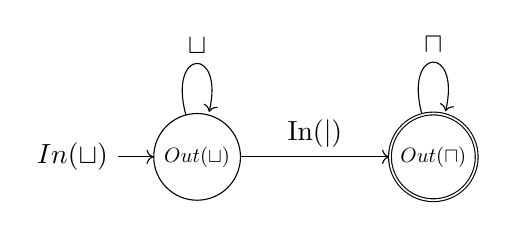
\begin{tikzpicture}                                                           
\ctikzset{->, .=stealth',tripoles/american or port/input height=.5,           
           node distance=3cm, initial text=$In(\sqcup)$ }          
\node[state, initial, scale=.75] (q1) {$ Out(\sqcup)$};           
\node[state, accepting, right of=q1, scale=.75] (q2) {$Out(\sqcap)$};
\draw (q1) edge[loop above] node{$\sqcup$} (q1)                        
(q1) edge[above] node{In($|$)} (q2)                            
(q2) edge[loop above] node{$\sqcap$} (q2);                                 
\end{tikzpicture}                                                             
\caption{Space State Diagram for OR Gate Circuit for Simple Latch Equation    
($\operatorname{In_{\sqcap}}{\left(t \right)} \subset \operatorname{Out_{\sqcap}}{\left(t \right)}$)}                                                      
\label{fig:Figure 9}                                                          
\end{figure}
The simple latch could be expressed as follows.
\begin{equation}
 \begin{minipage}{250pt}
\begin{flushleft} $\displaystyle Out=\begin{cases}    \sqcup & \\ \text{for}\: In \cup Out = \sqcup \\ \ \\    \sqcap & \\ \: otherwise \end{cases}$  \end{flushleft}
 \end{minipage}
 \end{equation}
\section{SR Flipflop}
Let the signals S and R be generated such that they are disjoint. Let S     input set the latched signal QS and let R input reset the latched signal     QS. Let the QR be the inverse of QS. Given these condition, the circuit     was derived as follows.
\begin{equation}
 \begin{minipage}{250pt}
\begin{flushleft} $\displaystyle S = \begin{cases} 0 & \\  \text{for}\: \left(t \geq 0 \wedge t < 6\right) \vee \left(t \geq 9 \wedge t < 13\right) \\ \quad \ \  \vee \left(t \geq 17 \wedge t < 18\right) \vee \left(t \geq 24 \wedge t < 28\right) \\ \quad \ \  \vee \left(t \geq 30 \wedge t < 60\right) \vee \left(t \geq 64 \wedge t < 67\right) \\ \quad \ \  \vee \left(t \geq 70 \wedge t < 71\right) \vee \left(t \geq 74 \wedge t < 78\right) \\ \quad \ \  \vee \left(t \geq 85 \wedge t < 88\right) \\1 & \\  \text{otherwise} \end{cases}$  \end{flushleft}
 \end{minipage}
 \end{equation}
\begin{table}[H] \caption{Signal S Pulses}\centering\begin{tabular}{|p{.4cm}|p{.5cm}|p{6.5cm}|}\hline Item&Pulse &Stem Set\\ \hline 00& \footnotesize$\sqcap$ & \footnotesize[7, 14, 15, 19, 20, 21, 22, 61, 62, 68, 72, 79, 80, 81, 82, 83]\\ \hline 01& \footnotesize$\sqcup$ & \footnotesize[1, 2, 3, 4, 10, 11, 25, 26, 31, 32, 33, 34, 35, 36, 37, 38, 39, 40, 41, 42, 43, 44, 45, 46, 47, 48, 49, 50, 51, 52, 53, 54, 55, 56, 57, 58, 65, 75, 76, 86]\\ \hline 02& \footnotesize$\nearrow$ & \footnotesize[6, 13, 18, 28, 60, 67, 71, 78]\\ \hline 03& \footnotesize$\searrow$ & \footnotesize[9, 24, 30, 64, 74, 85]\\ \hline 04& \footnotesize$\bot$ & \footnotesize[]\\ \hline 05& \footnotesize$\top$ & \footnotesize[17, 70]\\ \hline 06& \footnotesize$.\nearrow$ & \footnotesize[5, 12, 27, 59, 66, 77]\\ \hline 07& \footnotesize$^.\searrow$ & \footnotesize[8, 16, 23, 29, 63, 69, 73, 84]\\ \hline 08& \footnotesize$|$ & \footnotesize[6, 9, 13, 17, 18, 24, 28, 30, 60, 64, 67, 70, 71, 74, 78, 85]\\ \hline \end{tabular} \end{table} 
\begin{equation}
 \begin{minipage}{250pt}
\begin{flushleft} $\displaystyle R = \begin{cases} 0 & \\  \text{for}\: \left(t \geq 0 \wedge t < 36\right) \vee \left(t \geq 39 \wedge t < 42\right) \\ \quad \ \  \vee \left(t \geq 45 \wedge t < 46\right) \vee \left(t \geq 49 \wedge t < 52\right) \\ \quad \ \  \vee \left(t \geq 54 \wedge t < 90\right) \vee \left(t \geq 92 \wedge t < 99\right) \\ \quad \ \  \vee \left(t \geq 100 \wedge t < 101\right) \vee \left(t \geq 102 \wedge t < 104\right) \\1 & \\  \text{otherwise} \end{cases}$  \end{flushleft}
 \end{minipage}
 \end{equation}
\begin{table}[H] \caption{Signal R Pulses}\centering\begin{tabular}{|p{.4cm}|p{.5cm}|p{6.5cm}|}\hline Item&Pulse &Stem Set\\ \hline 00& \footnotesize$\sqcap$ & \footnotesize[37, 43, 47, 105]\\ \hline 01& \footnotesize$\sqcup$ & \footnotesize[1, 2, 3, 4, 5, 6, 7, 8, 9, 10, 11, 12, 13, 14, 15, 16, 17, 18, 19, 20, 21, 22, 23, 24, 25, 26, 27, 28, 29, 30, 31, 32, 33, 34, 40, 50, 55, 56, 57, 58, 59, 60, 61, 62, 63, 64, 65, 66, 67, 68, 69, 70, 71, 72, 73, 74, 75, 76, 77, 78, 79, 80, 81, 82, 83, 84, 85, 86, 87, 88, 93, 94, 95, 96, 97]\\ \hline 02& \footnotesize$\nearrow$ & \footnotesize[36, 42, 46, 52, 90, 104]\\ \hline 03& \footnotesize$\searrow$ & \footnotesize[39, 49, 54, 92, 102]\\ \hline 04& \footnotesize$\bot$ & \footnotesize[99, 101]\\ \hline 05& \footnotesize$\top$ & \footnotesize[45, 100]\\ \hline 06& \footnotesize$.\nearrow$ & \footnotesize[35, 41, 51, 89, 98, 103]\\ \hline 07& \footnotesize$^.\searrow$ & \footnotesize[38, 44, 48, 53, 91]\\ \hline 08& \footnotesize$|$ & \footnotesize[36, 39, 42, 45, 46, 49, 52, 54, 90, 92, 99, 100, 101, 102, 104]\\ \hline \end{tabular} \end{table} 
The output signal QS and QR were constructed as follows.
\begin{equation}
 \begin{minipage}{250pt}
\begin{flushleft} $\displaystyle QS = \begin{cases} 0 & \text{for}\: \left(t \geq 0 \wedge t < 6\right) \vee \left(t \geq 37 \wedge t < 60\right) \\1 & \text{otherwise} \end{cases}$  \end{flushleft}
 \end{minipage}
 \end{equation}
\begin{table}[H] \caption{Signal QS Pulses}\centering\begin{tabular}{|p{.4cm}|p{.5cm}|p{6.5cm}|}\hline Item&Pulse &Stem Set\\ \hline 00& \footnotesize$\sqcap$ & \footnotesize[7, 8, 9, 10, 11, 12, 13, 14, 15, 16, 17, 18, 19, 20, 21, 22, 23, 24, 25, 26, 27, 28, 29, 30, 31, 32, 33, 34, 35, 61, 62, 63, 64, 65, 66, 67, 68, 69, 70, 71, 72, 73, 74, 75, 76, 77, 78, 79, 80, 81, 82, 83, 84, 85, 86, 87, 88, 89, 90, 91, 92, 93, 94, 95, 96, 97, 98, 99, 100, 101, 102, 103, 104, 105, 106, 107, 108]\\ \hline 01& \footnotesize$\sqcup$ & \footnotesize[1, 2, 3, 4, 38, 39, 40, 41, 42, 43, 44, 45, 46, 47, 48, 49, 50, 51, 52, 53, 54, 55, 56, 57, 58]\\ \hline 02& \footnotesize$\nearrow$ & \footnotesize[6, 60]\\ \hline 03& \footnotesize$\searrow$ & \footnotesize[37]\\ \hline 04& \footnotesize$\bot$ & \footnotesize[]\\ \hline 05& \footnotesize$\top$ & \footnotesize[]\\ \hline 06& \footnotesize$.\nearrow$ & \footnotesize[5, 59]\\ \hline 07& \footnotesize$^.\searrow$ & \footnotesize[36]\\ \hline 08& \footnotesize$|$ & \footnotesize[6, 37, 60]\\ \hline \end{tabular} \end{table} 
\begin{equation}
 \begin{minipage}{250pt}
\begin{flushleft} $\displaystyle QR = \begin{cases} 1 & \\  \text{for}\: \left(t \geq 0 \wedge t < 7\right) \vee \left(t \geq 36 \wedge t < 61\right) \\ \quad \ \  \vee \left(t \geq 90 \wedge t < 92\right) \vee \left(t \geq 99 \wedge t < 100\right) \\ \quad \ \  \vee \left(t \geq 101 \wedge t < 102\right) \vee \left(t \geq 104 \wedge t < 110\right) \\0 & \\  \text{otherwise} \end{cases}$  \end{flushleft}
 \end{minipage}
 \end{equation}
\begin{table}[H] \caption{Signal QR Pulses}\centering\begin{tabular}{|p{.4cm}|p{.5cm}|p{6.5cm}|}\hline Item&Pulse &Stem Set\\ \hline 00& \footnotesize$\sqcap$ & \footnotesize[1, 2, 3, 4, 5, 37, 38, 39, 40, 41, 42, 43, 44, 45, 46, 47, 48, 49, 50, 51, 52, 53, 54, 55, 56, 57, 58, 59, 105, 106, 107, 108]\\ \hline 01& \footnotesize$\sqcup$ & \footnotesize[8, 9, 10, 11, 12, 13, 14, 15, 16, 17, 18, 19, 20, 21, 22, 23, 24, 25, 26, 27, 28, 29, 30, 31, 32, 33, 34, 62, 63, 64, 65, 66, 67, 68, 69, 70, 71, 72, 73, 74, 75, 76, 77, 78, 79, 80, 81, 82, 83, 84, 85, 86, 87, 88, 93, 94, 95, 96, 97]\\ \hline 02& \footnotesize$\nearrow$ & \footnotesize[36, 90, 104]\\ \hline 03& \footnotesize$\searrow$ & \footnotesize[7, 61, 92, 102]\\ \hline 04& \footnotesize$\bot$ & \footnotesize[99, 101]\\ \hline 05& \footnotesize$\top$ & \footnotesize[100]\\ \hline 06& \footnotesize$.\nearrow$ & \footnotesize[35, 89, 98, 103]\\ \hline 07& \footnotesize$^.\searrow$ & \footnotesize[6, 60, 91]\\ \hline 08& \footnotesize$|$ & \footnotesize[7, 36, 61, 90, 92, 99, 100, 101, 102, 104]\\ \hline \end{tabular} \end{table} 
The signals S, R, QS and QR were plotted in Figure 10.
\begin{figure}[H]
\centering\includegraphics[width=1\linewidth,height=0.35\textheight]{FG010.png}
\caption{SR Flipflop Timing Diagram}
\label{fig:FG010.png}
\end{figure}

\subsection{SR Model}
By inspection of S and QS in Figure 10, the following was observed.
\begin{equation}
 \begin{minipage}{250pt}
\begin{flushleft} $\displaystyle S_{\sqcap} \subset QS_{\sqcap}$  \end{flushleft}
 \end{minipage}
 \end{equation}
Transforming (37) into an equation,
\begin{equation}
 \begin{minipage}{250pt}
\begin{flushleft} $\displaystyle QS_{\sqcap} = QS_{\sqcap}  \cup  S_{\sqcap}$  \end{flushleft}
 \end{minipage}
 \end{equation}
Likewise inspecting R and QR, 
\begin{equation}
 \begin{minipage}{250pt}
\begin{flushleft} $\displaystyle R_{\sqcap} \subset QR_{\sqcap}$  \end{flushleft}
 \end{minipage}
 \end{equation}
Transforming (39) into an equation,
\begin{equation}
 \begin{minipage}{250pt}
\begin{flushleft} $\displaystyle QR_{\sqcap} = QR_{\sqcap}  \cup  R_{\sqcap}$  \end{flushleft}
 \end{minipage}
 \end{equation}
The relationship of QS and QR was established as follows.
\begin{equation}
 \begin{minipage}{250pt}
\begin{flushleft} $\displaystyle \operatorname{I_{nv}}{\left(QS_{\sqcap} \right)} = QR_{\sqcap} = \overline{QS_{\sqcap}}$  \end{flushleft}
 \end{minipage}
 \end{equation}
\begin{equation}
 \begin{minipage}{250pt}
\begin{flushleft} $\displaystyle \operatorname{I_{nv}}{\left(QR_{\sqcap} \right)} = QS_{\sqcap} = \overline{QR_{\sqcap}}$  \end{flushleft}
 \end{minipage}
 \end{equation}
Substituting (42) in the right hand side of (38) and  (41) in the right hand side of (40),  
\begin{equation}
 \begin{minipage}{250pt}
\begin{flushleft} $\displaystyle QS_{\sqcap} = S_{\sqcap}  \cup  \overline{QR_{\sqcap}}$  \end{flushleft}
 \end{minipage}
 \end{equation}
\begin{equation}
 \begin{minipage}{250pt}
\begin{flushleft} $\displaystyle QR_{\sqcap} = R_{\sqcap}  \cup  \overline{QS_{\sqcap}}$  \end{flushleft}
 \end{minipage}
 \end{equation}
\subsection{SR Flipflop Circuit}
The equations (43) and (44) were realized     through the circuit diagram in Figure 11. The OR gate was the union     operation in set theory, the equivalent addition (+) operation in Boolean     algebra.
\begin{figure}[H]                                                             
    \centering                                                                
	\tikzstyle{block} = [draw, fill=white, rectangle,                         
	minimum height=1.5cm, minimum width=3cm]                                   
	\tikzstyle{input} = [coordinate]                                          
	\tikzstyle{output} = [coordinate]                                         
	\tikzstyle{pinstyle} = [pin edge={to-,thin,black}]                        
\begin{circuitikz}                                                            
\ctikzset{tripoles/american or port/input height=.5}                          
\node[input,name=S] {$S$};                                                    
\node[input,below of =S, name=R, node distance=3.5cm] {$R$};                  
\node[american or port,right of = S,anchor=in 1,node distance=1cm] (ORs) {};  
\node[american or port,right of = R,anchor=in 2,node distance=1cm] (ORr) {};  
\node[american not port,below of=ORs,rotate=180,scale=.5,node distance=1cm](Is){};
\node[american not port,above of=ORr,rotate=180,scale=.5,node distance=1cm](Ir){};
\node[output, left of = Is, node distance=1cm] (fs){};                        
\node[output, left of = Ir, node distance=1cm] (fr){};                        
\node[output, right of=ORs, node distance=.5cm] (Qs) {$QS$}; 
\node[output, right of=ORr, node distance=.5cm] (Qr) {$QR$}; 
\draw (ORs.out) -- (Qs) node{$\quad\quad QS_{\sqcap}$} -|  (Is.in); 
\draw (ORr.out) -- (Qr) node{$\quad\quad QR_{\sqcap}$} -| (Ir.in); 
\draw (Is.out) -- (fs)  -- (ORr.in 1) node {$\overline{QS_{\sqcap}}\quad\quad\quad$}; 
\draw (Ir.out) -- (fr) -- (ORs.in 2) node {$\overline{QR_{\sqcap}}\quad\quad\quad$}; 
\draw  (S) node {$S_{\sqcap}\quad\quad$}-- (ORs.in 1); 
\draw  (R) node {$R_{\sqcap}\quad\quad$}-- (ORr.in 2); 
\end{circuitikz} 
\caption{OR Gate Circuit for SR Flipflop} 
\label{fig:Figure 11}                                                 
\end{figure}
Note that intersecting (37) with (39), 
\begin{equation}
 \begin{minipage}{250pt}
\begin{flushleft} $\displaystyle S_{\sqcap} \wedge R_{\sqcap} \subset QS_{\sqcap} \wedge QR_{\sqcap} = null = \phi$  \end{flushleft}
 \end{minipage}
 \end{equation}
Therefore, the disjoint feature of S and R must be maintained to keep the     SR Flipflop operating in latching function. However, S and R may not be     kept disjoint for practical reasonss. \\ \ \\ 
Hence, the set equation of SR flipflop was expressed as follows.
\begin{equation}
 \begin{minipage}{250pt}
\begin{flushleft} $\displaystyle \left[\begin{matrix}QS\\QR\end{matrix}\right]=\begin{cases} \left[\begin{matrix}S\\R\end{matrix}\right] \cup \left[\begin{matrix}\overline{QR}\\\overline{QS}\end{matrix}\right] & \text{for}\: S \cap R = \phi \\ \ \\ \left[\begin{matrix}QS\\QR\end{matrix}\right] & \text{for}\: S \cup R = \phi \end{cases}$  \end{flushleft}
 \end{minipage}
 \end{equation}
\subsection{Model of Cross Coupled OR Gate SR Flipflop}
The cross coupled OR Gate SR Flipflop behaved differently when      the non-disjoint signals S and R were inputted. Let's consider the following     non-disjoint signals.
\begin{equation}
 \begin{minipage}{250pt}
\begin{flushleft} $\displaystyle S = \begin{cases} 1 & \\  \text{for}\: \left(t \geq 0 \wedge t < 10\right) \vee \left(t \geq 20 \wedge t <23 \right) \\ \quad \ \  \vee \left(t \geq 24 \wedge t < 28\right) \vee \left(t \geq 65 \wedge t <66 \right) \\ \quad \ \  \vee \left(t \geq 88 \wedge t < 89\right) \vee \left(t \geq 100 \wedge t < 102\right) \\ \quad \ \  \vee \left(t \geq 105 \wedge t < 106\right) \vee \left(t \geq 115 \wedge t < 116\right) \\ \quad \ \  \vee \left(t \geq 125 \wedge t < 130\right) \vee \left(t \geq 131 \wedge t < 141\right) \\ \quad \ \  \vee \left(t \geq 142 \wedge t < 160\right) \\0 & \\  \text{otherwise} \end{cases}$  \end{flushleft}
 \end{minipage}
 \end{equation}
\begin{table}[H] \caption{Signal S Pulses}\centering\begin{tabular}{|p{.4cm}|p{.5cm}|p{6.5cm}|}\hline Item&Pulse &Stem Set\\ \hline 00& \footnotesize$\sqcap$ & \footnotesize[1, 2, 3, 4, 5, 6, 7, 8, 21, 25, 26, 126, 127, 128, 132, 133, 134, 135, 136, 137, 138, 139, 143, 144, 145, 146, 147, 148, 149, 150, 151, 152, 153, 154, 155, 156, 157, 158]\\ \hline 01& \footnotesize$\sqcup$ & \footnotesize[11, 12, 13, 14, 15, 16, 17, 18, 29, 30, 31, 32, 33, 34, 35, 36, 37, 38, 39, 40, 41, 42, 43, 44, 45, 46, 47, 48, 49, 50, 51, 52, 53, 54, 55, 56, 57, 58, 59, 60, 61, 62, 63, 67, 68, 69, 70, 71, 72, 73, 74, 75, 76, 77, 78, 79, 80, 81, 82, 83, 84, 85, 86, 90, 91, 92, 93, 94, 95, 96, 97, 98, 103, 107, 108, 109, 110, 111, 112, 113, 117, 118, 119, 120, 121, 122, 123]\\ \hline 02& \footnotesize$\nearrow$ & \footnotesize[20, 24, 100, 125, 131, 142]\\ \hline 03& \footnotesize$\searrow$ & \footnotesize[10, 28, 66, 89, 102, 106, 116]\\ \hline 04& \footnotesize$\bot$ & \footnotesize[65, 88, 105, 115]\\ \hline 05& \footnotesize$\top$ & \footnotesize[23, 130, 141]\\ \hline 06& \footnotesize$.\nearrow$ & \footnotesize[19, 64, 87, 99, 104, 114, 124]\\ \hline 07& \footnotesize$^.\searrow$ & \footnotesize[9, 22, 27, 101, 129, 140]\\ \hline 08& \footnotesize$|$ & \footnotesize[10, 20, 23, 24, 28, 65, 66, 88, 89, 100, 102, 105, 106, 115, 116, 125, 130, 131, 141, 142]\\ \hline \end{tabular} \end{table} 
\begin{equation}
 \begin{minipage}{250pt}
\begin{flushleft} $\displaystyle R = \begin{cases} 1 & \\  \text{for}\: \left(t \geq 0 \wedge t < 10\right) \vee \left(t \geq 35 \wedge t <36 \right) \\ \quad \ \  \vee \left(t \geq 50 \wedge t < 53\right) \vee \left(t \geq 54 \wedge t <58 \right) \\ \quad \ \  \vee \left(t \geq 75 \wedge t < 78\right) \vee \left(t \geq 80 \wedge t <83\right) \\ \quad \ \  \vee \left(t \geq 88 \wedge t < 89\right) \vee \left(t \geq 115 \wedge t < 116\right) \\ \quad \ \  \vee \left(t \geq 125 \wedge t < 130\right) \vee \left(t \geq 131 \wedge t < 150\right) \\ \quad \ \  \vee \left(t \geq 151 \wedge t < 160\right) \\0 & \\  \text{otherwise} \end{cases}$  \end{flushleft}
 \end{minipage}
 \end{equation}
\begin{table}[H] \caption{Signal R Pulses}\centering\begin{tabular}{|p{.4cm}|p{.5cm}|p{6.5cm}|}\hline Item&Pulse &Stem Set\\ \hline 00& \footnotesize$\sqcap$ & \footnotesize[1, 2, 3, 4, 5, 6, 7, 8, 51, 55, 56, 76, 81, 126, 127, 128, 132, 133, 134, 135, 136, 137, 138, 139, 140, 141, 142, 143, 144, 145, 146, 147, 148, 152, 153, 154, 155, 156, 157, 158]\\ \hline 01& \footnotesize$\sqcup$ & \footnotesize[11, 12, 13, 14, 15, 16, 17, 18, 19, 20, 21, 22, 23, 24, 25, 26, 27, 28, 29, 30, 31, 32, 33, 37, 38, 39, 40, 41, 42, 43, 44, 45, 46, 47, 48, 59, 60, 61, 62, 63, 64, 65, 66, 67, 68, 69, 70, 71, 72, 73, 84, 85, 86, 90, 91, 92, 93, 94, 95, 96, 97, 98, 99, 100, 101, 102, 103, 104, 105, 106, 107, 108, 109, 110, 111, 112, 113, 117, 118, 119, 120, 121, 122, 123]\\ \hline 02& \footnotesize$\nearrow$ & \footnotesize[50, 54, 75, 80, 125, 131, 151]\\ \hline 03& \footnotesize$\searrow$ & \footnotesize[10, 36, 58, 78, 83, 89, 116]\\ \hline 04& \footnotesize$\bot$ & \footnotesize[35, 88, 115]\\ \hline 05& \footnotesize$\top$ & \footnotesize[53, 130, 150]\\ \hline 06& \footnotesize$.\nearrow$ & \footnotesize[34, 49, 74, 79, 87, 114, 124]\\ \hline 07& \footnotesize$^.\searrow$ & \footnotesize[9, 52, 57, 77, 82, 129, 149]\\ \hline 08& \footnotesize$|$ & \footnotesize[10, 35, 36, 50, 53, 54, 58, 75, 78, 80, 83, 88, 89, 115, 116, 125, 130, 131, 150, 151]\\ \hline \end{tabular} \end{table} 
\begin{equation}
 \begin{minipage}{250pt}
\begin{flushleft} $\displaystyle QS = \begin{cases} 1 & \\  \text{for}\: \left(t \geq 0 \wedge t < 10\right) \vee \left(t \geq 11 \wedge t < 12 \right) \\ \quad \ \  \vee \left(t \geq 13 \wedge t < 14\right) \vee \left(t \geq 15 \wedge t < 16 \right) \\ \quad \ \  \vee \left(t \geq 17 \wedge t < 18\right) \vee \left(t \geq 19 \wedge t < 36\right) \\ \quad \ \  \vee \left(t \geq 37 \wedge t < 38\right) \vee \left(t \geq 39 \wedge t < 40\right) \\ \quad \ \  \vee \left(t \geq 41 \wedge t < 42\right) \vee \left(t \geq 43 \wedge t < 44\right) \\ \quad \ \  \vee \left(t \geq 45 \wedge t < 46\right) \vee \left(t \geq 47 \wedge t < 48\right) \\ \quad \ \  \vee \left(t \geq 49 \wedge t < 50\right) \vee \left(t \geq 65 \wedge t < 66 \right) \\ \quad \ \  \vee \left(t \geq 67 \wedge t < 68\right) \vee \left(t \geq 69 \wedge t < 70\right) \\ \quad \ \  \vee \left(t \geq 71 \wedge t < 72\right) \vee \left(t \geq 73 \wedge t < 74\right) \\ \quad \ \  \vee \left(t \geq 75 \wedge t < 76\right) \vee \left(t \geq 88 \wedge t < 89 \right) \\ \quad \ \  \vee \left(t \geq 90 \wedge t < 91\right) \vee \left(t \geq 92 \wedge t < 93\right) \\ \quad \ \  \vee \left(t \geq 94 \wedge t < 95\right) \vee \left(t \geq 96 \wedge t < 97\right) \\ \quad \ \  \vee \left(t \geq 98 \wedge t < 99\right) \vee \left(t \geq 100 \wedge t < 116\right) \\ \quad \ \  \vee \left(t \geq 117 \wedge t < 118\right) \vee \left(t \geq 119 \wedge t < 120 \right) \\ \quad \ \  \vee \left(t \geq 121 \wedge t < 122\right) \vee \left(t \geq 123 \wedge t < 124\right) \\ \quad \ \  \vee \left(t \geq 125 \wedge t < 130\right) \vee \left(t \geq 131 \wedge t < 141\right) \\ \quad \ \  \vee \left(t \geq 142 \wedge t < 160\right) \\0 & \\  \text{otherwise} \end{cases}$  \end{flushleft}
 \end{minipage}
 \end{equation}
\begin{table}[H] \caption{Signal QS Pulses}\centering\begin{tabular}{|p{.4cm}|p{.5cm}|p{6.5cm}|}\hline Item&Pulse &Stem Set\\ \hline 00& \footnotesize$\sqcap$ & \footnotesize[1, 2, 3, 4, 5, 6, 7, 8, 20, 21, 22, 23, 24, 25, 26, 27, 28, 29, 30, 31, 32, 33, 34, 101, 102, 103, 104, 105, 106, 107, 108, 109, 110, 111, 112, 113, 114, 126, 127, 128, 132, 133, 134, 135, 136, 137, 138, 139, 143, 144, 145, 146, 147, 148, 149, 150, 151, 152, 153, 154, 155, 156, 157, 158]\\ \hline 01& \footnotesize$\sqcup$ & \footnotesize[51, 52, 53, 54, 55, 56, 57, 58, 59, 60, 61, 62, 63, 77, 78, 79, 80, 81, 82, 83, 84, 85, 86]\\ \hline 02& \footnotesize$\nearrow$ & \footnotesize[19, 100, 125, 131, 142]\\ \hline 03& \footnotesize$\searrow$ & \footnotesize[50, 76]\\ \hline 04& \footnotesize$\bot$ & \footnotesize[11, 13, 15, 17, 37, 39, 41, 43, 45, 47, 49, 65, 67, 69, 71, 73, 75, 88, 90, 92, 94, 96, 98, 117, 119, 121, 123]\\ \hline 05& \footnotesize$\top$ & \footnotesize[10, 12, 14, 16, 18, 36, 38, 40, 42, 44, 46, 48, 66, 68, 70, 72, 74, 89, 91, 93, 95, 97, 99, 116, 118, 120, 122, 124, 130, 141]\\ \hline 06& \footnotesize$.\nearrow$ & \footnotesize[64, 87]\\ \hline 07& \footnotesize$^.\searrow$ & \footnotesize[9, 35, 115, 129, 140]\\ \hline 08& \footnotesize$|$ & \footnotesize[10, 11, 12, 13, 14, 15, 16, 17, 18, 19, 36, 37, 38, 39, 40, 41, 42, 43, 44, 45, 46, 47, 48, 49, 50, 65, 66, 67, 68, 69, 70, 71, 72, 73, 74, 75, 76, 88, 89, 90, 91, 92, 93, 94, 95, 96, 97, 98, 99, 100, 116, 117, 118, 119, 120, 121, 122, 123, 124, 125, 130, 131, 141, 142]\\ \hline \end{tabular} \end{table} 
\begin{equation}
 \begin{minipage}{250pt}
\begin{flushleft} $\displaystyle QR = \begin{cases} 1 & \\  \text{for}\: \left(t \geq 0 \wedge t < 10\right) \vee \left(t \geq 11 \wedge t < 12 \right) \\ \quad \ \  \vee \left(t \geq 13 \wedge t < 14\right) \vee \left(t \geq 15 \wedge t < 16 \right) \\ \quad \ \  \vee \left(t \geq 17 \wedge t < 18\right) \vee \left(t \geq 19 \wedge t < 20\right) \\ \quad \ \  \vee \left(t \geq 35 \wedge t < 36\right) \vee \left(t \geq 37 \wedge t < 38\right) \\ \quad \ \  \vee \left(t \geq 39 \wedge t < 40\right) \vee \left(t \geq 41 \wedge t < 42\right) \\ \quad \ \  \vee \left(t \geq 43 \wedge t < 44\right) \vee \left(t \geq 45 \wedge t < 46\right) \\ \quad \ \  \vee \left(t \geq 47 \wedge t < 48\right) \vee \left(t \geq 49 \wedge t < 66 \right) \\ \quad \ \  \vee \left(t \geq 67 \wedge t < 68\right) \vee \left(t \geq 69 \wedge t < 70\right) \\ \quad \ \  \vee \left(t \geq 71 \wedge t < 72\right) \vee \left(t \geq 73 \wedge t < 74\right) \\ \quad \ \  \vee \left(t \geq 75 \wedge t < 89\right) \vee \left(t \geq 90 \wedge t < 91 \right) \\ \quad \ \  \vee \left(t \geq 92 \wedge t < 93\right) \vee \left(t \geq 94 \wedge t < 95\right) \\ \quad \ \  \vee \left(t \geq 96 \wedge t < 97\right) \vee \left(t \geq 98 \wedge t < 99\right) \\ \quad \ \  \vee \left(t \geq 100 \wedge t < 101\right) \vee \left(t \geq 115 \wedge t < 116\right) \\ \quad \ \  \vee \left(t \geq 117 \wedge t < 118\right) \vee \left(t \geq 119 \wedge t < 120 \right) \\ \quad \ \  \vee \left(t \geq 121 \wedge t < 122\right) \vee \left(t \geq 123 \wedge t < 124\right) \\ \quad \ \  \vee \left(t \geq 125 \wedge t < 130\right) \vee \left(t \geq 131 \wedge t < 150\right) \\ \quad \ \  \vee \left(t \geq 151 \wedge t < 160\right) \\0 & \\  \text{otherwise} \end{cases}$  \end{flushleft}
 \end{minipage}
 \end{equation}
\begin{table}[H] \caption{Signal QR Pulses}\centering\begin{tabular}{|p{.4cm}|p{.5cm}|p{6.5cm}|}\hline Item&Pulse &Stem Set\\ \hline 00& \footnotesize$\sqcap$ & \footnotesize[1, 2, 3, 4, 5, 6, 7, 8, 50, 51, 52, 53, 54, 55, 56, 57, 58, 59, 60, 61, 62, 63, 64, 76, 77, 78, 79, 80, 81, 82, 83, 84, 85, 86, 87, 126, 127, 128, 132, 133, 134, 135, 136, 137, 138, 139, 140, 141, 142, 143, 144, 145, 146, 147, 148, 152, 153, 154, 155, 156, 157, 158]\\ \hline 01& \footnotesize$\sqcup$ & \footnotesize[21, 22, 23, 24, 25, 26, 27, 28, 29, 30, 31, 32, 33, 102, 103, 104, 105, 106, 107, 108, 109, 110, 111, 112, 113]\\ \hline 02& \footnotesize$\nearrow$ & \footnotesize[49, 75, 125, 131, 151]\\ \hline 03& \footnotesize$\searrow$ & \footnotesize[20, 101]\\ \hline 04& \footnotesize$\bot$ & \footnotesize[11, 13, 15, 17, 19, 35, 37, 39, 41, 43, 45, 47, 67, 69, 71, 73, 90, 92, 94, 96, 98, 100, 115, 117, 119, 121, 123]\\ \hline 05& \footnotesize$\top$ & \footnotesize[10, 12, 14, 16, 18, 36, 38, 40, 42, 44, 46, 48, 66, 68, 70, 72, 74, 89, 91, 93, 95, 97, 99, 116, 118, 120, 122, 124, 130, 150]\\ \hline 06& \footnotesize$.\nearrow$ & \footnotesize[34, 114]\\ \hline 07& \footnotesize$^.\searrow$ & \footnotesize[9, 65, 88, 129, 149]\\ \hline 08& \footnotesize$|$ & \footnotesize[10, 11, 12, 13, 14, 15, 16, 17, 18, 19, 20, 35, 36, 37, 38, 39, 40, 41, 42, 43, 44, 45, 46, 47, 48, 49, 66, 67, 68, 69, 70, 71, 72, 73, 74, 75, 89, 90, 91, 92, 93, 94, 95, 96, 97, 98, 99, 100, 101, 115, 116, 117, 118, 119, 120, 121, 122, 123, 124, 125, 130, 131, 150, 151]\\ \hline \end{tabular} \end{table} 
Applying the signals from (47) and (48) to OR Gated    SR flipflop, the timing diagram behavior was generated as shown in Figure 12.    The space state diagram for Figure 12 timing diagram was depicted in Figure 13.
\begin{figure}[H]
\centering\includegraphics[width=1\linewidth,height=0.35\textheight]{FG012.png}
\caption{Non-disjoint S and R Signals SR Flipflop Timing Diagram}
\label{fig:FG012.png}
\end{figure}

\begin{figure}[H]                                                                
\centering                                                                       
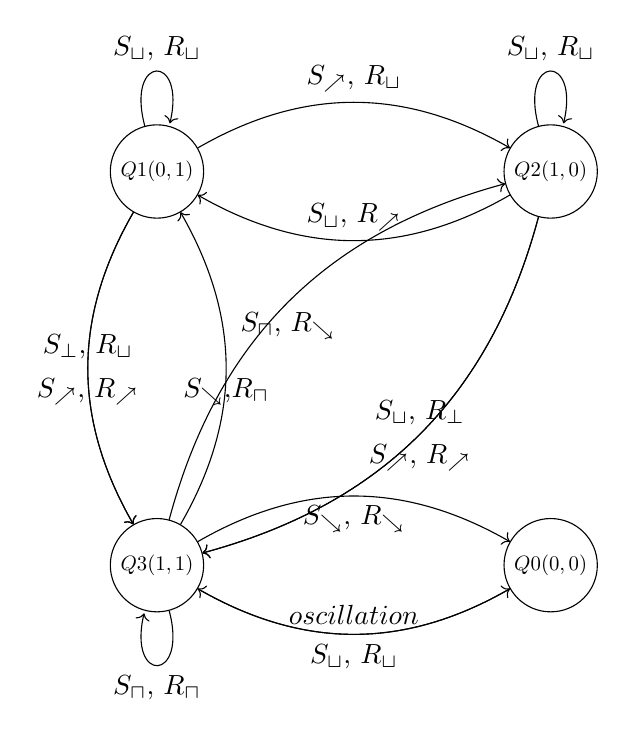
\begin{tikzpicture}                                                              
\ctikzset{->,.=stealth',tripoles/american or port/input height=.5,               
           node distance=2cm, initial text=$$ }                                   
\node[state,                scale=.75,  node distance=5cm](q1){$Q1(0,1)$};       
\node[state, right of = q1, scale=.75,  node distance=5cm](q2){$Q2(1,0)$};       
\node[state, below of = q1, scale=.75,  node distance=5cm](q3){$Q3(1,1)$};       
\node[state, right of = q3, scale=.75,  node distance=5cm](q0){$Q0(0,0)$};       
\draw (q0) edge[bend left,  below] node{$S_{\sqcup}$, $R_{\sqcup}$} (q3);
\draw (q1) edge[loop        above] node{$S_{\sqcup}$, $R_{\sqcup}$}      
(q1) edge[bend left,         above] node{$S_{\nearrow}$, $R_{\sqcup}$} (q2) 
(q1) edge[bend right,        above] node{$S_{\bot}$, $R_{\sqcup}$} (q3) 
(q1) edge[bend right,        below] node{$S_{\nearrow}$, $R_{\nearrow}$} (q3);
\draw (q2) edge[loop        above] node{$S_{\sqcup}$, $R_{\sqcup}$}      
(q2) edge[bend left,         above] node{$S_{\sqcup}$, $R_{\nearrow}$} (q1) 
(q2) edge[bend left,         below] node{$S_{\nearrow}$, $R_{\nearrow}$} (q3) 
(q2) edge[bend left,         above] node{$S_{\sqcup}$, $R_{\bot}$} (q3);
\draw (q3) edge[loop        below] node{$S_{\sqcap}$, $R_{\sqcap}$}            
(q3) edge[bend left,         below] node{$S_{\searrow}$, $R_{\searrow}$} (q0) 
(q3) edge[bend right,        above] node{$oscillation$}                      (q0) 
(q3) edge[bend right,        below] node{$S_{\searrow}$,$R_{\sqcap}$} (q1) 
(q3) edge[bend left,         below] node{$S_{\sqcap}$, $R_{\searrow}$} (q2);
\end{tikzpicture}                                                                
\caption{Space State Diagram SR Flipflop Operation in Figure 12 }                
\label{fig:Figure 13}                                                            
\end{figure}
\subsection{Symbolic Pulses Features}
The symbolic pulses were related as follows.  
\begin{equation}
 \begin{minipage}{250pt}
\begin{flushleft} $\displaystyle \sqcap\supset {\nearrow\cup.\nearrow\cup\searrow\cup^.\searrow\cup\bot\cup\top\cup|\cup\sqcup}$  \end{flushleft}
 \end{minipage}
 \end{equation}
Given a set of 5-stem sequence, it could be represented by a sequence of    the symbolic pulses as shown in Table 1.
\begin{table}[H] \caption{Combination of a Three of Pulses in Four Time Points}\centering\begin{tabular}{|p{.5cm}|p{1.5cm}|p{3.85cm}|}\hline Items&Stems     &Pulses at Time Points \\ \end{tabular} \\ 
\begin{tabular}{|p{.5cm}|p{1.5cm}|p{1cm} p{1cm} p{1cm}|}&0,1,2,3,4 &1 &2 &3 \\ \hline 00&0,0,0,0,0 &$\sqcup$,&$\sqcup$,&$\sqcup$ \\ \hline 01&1,0,0,0,0 &$\searrow$,&$\sqcup$,&$\sqcup$ \\ \hline 02&0,1,0,0,0 &$\bot$,&$\searrow$,&$\sqcup$ \\ \hline 03&1,1,0,0,0 &$^.\searrow$,&$\searrow$,&$\sqcup$ \\ \hline 04&0,0,1,0,0 &$.\nearrow$,&$\bot$,&$\searrow$ \\ \hline 05&1,0,1,0,0 &$\top$,&$\bot$,&$\searrow$ \\ \hline 06&0,1,1,0,0 &$\nearrow$,&$^.\searrow$,&$\searrow$ \\ \hline 07&1,1,1,0,0 &$\sqcap$,&$^.\searrow$,&$\searrow$ \\ \hline 08&0,0,0,1,0 &$\sqcup$,&$.\nearrow$,&$\bot$ \\ \hline 09&1,0,0,1,0 &$\searrow$,&$.\nearrow$,&$\bot$ \\ \hline 10&0,1,0,1,0 &$\bot$,&$\top$,&$\bot$ \\ \hline 11&1,1,0,1,0 &$^.\searrow$,&$\top$,&$\bot$ \\ \hline 12&0,0,1,1,0 &$.\nearrow$,&$\nearrow$,&$^.\searrow$ \\ \hline 13&1,0,1,1,0 &$\top$,&$\nearrow$,&$^.\searrow$ \\ \hline 14&0,1,1,1,0 &$\nearrow$,&$\sqcap$,&$^.\searrow$ \\ \hline 15&1,1,1,1,0 &$\sqcap$,&$\sqcap$,&$^.\searrow$ \\ \hline 16&0,0,0,0,1 &$\sqcup$,&$\sqcup$,&$.\nearrow$ \\ \hline 17&1,0,0,0,1 &$\searrow$,&$\sqcup$,&$.\nearrow$ \\ \hline 18&0,1,0,0,1 &$\bot$,&$\searrow$,&$.\nearrow$ \\ \hline 19&1,1,0,0,1 &$^.\searrow$,&$\searrow$,&$.\nearrow$ \\ \hline 20&0,0,1,0,1 &$.\nearrow$,&$\bot$,&$\top$ \\ \hline 21&1,0,1,0,1 &$\top$,&$\bot$,&$\top$ \\ \hline 22&0,1,1,0,1 &$\nearrow$,&$^.\searrow$,&$\top$ \\ \hline 23&1,1,1,0,1 &$\sqcap$,&$^.\searrow$,&$\top$ \\ \hline 24&0,0,0,1,1 &$\sqcup$,&$.\nearrow$,&$\nearrow$ \\ \hline 25&1,0,0,1,1 &$\searrow$,&$.\nearrow$,&$\nearrow$ \\ \hline 26&0,1,0,1,1 &$\bot$,&$\top$,&$\nearrow$ \\ \hline 27&1,1,0,1,1 &$^.\searrow$,&$\top$,&$\nearrow$ \\ \hline 28&0,0,1,1,1 &$.\nearrow$,&$\nearrow$,&$\sqcap$ \\ \hline 28&1,0,1,1,1 &$\top$,&$\nearrow$,&$\sqcap$ \\ \hline 30&0,1,1,1,1 &$\nearrow$,&$\sqcap$,&$\sqcap$ \\ \hline 31&1,1,1,1,1 &$\sqcap$,&$\sqcap$,&$\sqcap$ \\ \hline \end{tabular} \end{table} 
\begin{table}[H] \caption{SR Flipflop in Oscillation Operation}\centering\begin{tabular}{|p{.3cm}|p{1.5cm}|p{5.5cm}|}\hline Item&Signals &Stems \\ \end{tabular} \\ \begin{tabular}{|p{.3cm}|p{1.5cm}|p{.1cm}|p{.1cm}|p{.3cm}|p{.47cm}|p{.1cm}                                  |p{.1cm}|p{.1cm}|p{.1cm}|p{.1cm}|p{.1cm}|}\hline 00&$S$ &1&1&1&0&0&0&0&0&0&0 \\    & & &$\sqcap$&$^.\searrow$&$\searrow$&$\sqcup$&$\sqcup$&$\sqcup$&$\sqcup$&$\sqcup$& \\ \hline 01&$\overline{QR}$ &0&0&0&0&1&0&1&0&1&0 \\    & & &$\sqcup$&$\sqcup$&$.\nearrow$&$\bot$&$\top$&$\bot$&$\top$&$\bot$& \\ \hline 02&$S$$\vee$$\overline{QR}$=$QS$&1&1&1&0&1&0&1&0&1&0 \\    & & &$\sqcap$&$^.\searrow$&$\top$&$\bot$&$\top$&$\bot$&$\top$&$\bot$& \\ \hline 03&$R$ &1&1&1&0&0&0&0&0&0&0 \\    & & &$\sqcap$&$^.\searrow$&$\searrow$&$\sqcup$&$\sqcup$&$\sqcup$&$\sqcup$&$\sqcup$& \\ \hline 04&$\overline{QS}$ &0&0&0&0&1&0&1&0&1&0 \\    & & &$\sqcup$&$\sqcup$&$.\nearrow$&$\bot$&$\top$&$\bot$&$\top$&$\bot$& \\ \hline 05&$R$$\vee$$\overline{QS}$=$QR$&1&1&1&0&1&0&1&0&1&0 \\    & & &$\sqcap$&$^.\searrow$&$\top$&$\bot$&$\top$&$\bot$&$\top$&$\bot$& \\ \hline \end{tabular} \end{table} 
At stead state of Q3(1,1), 
\begin{equation}
 \begin{minipage}{250pt}
\begin{flushleft} $\displaystyle \operatorname{QS}{\left(\sqcap \right)} = S{\left(\sqcap \right)} \cup \overline{QR}{\left(\sqcup \right)}$  \end{flushleft}
 \end{minipage}
 \end{equation}
\begin{equation}
 \begin{minipage}{250pt}
\begin{flushleft} $\displaystyle \operatorname{QR}{\left(\sqcap \right)} = R{\left(\sqcap \right)} \cup \overline{QS}{\left(\sqcup \right)}$  \end{flushleft}
 \end{minipage}
 \end{equation}
\subsection{Application of Event Property in SR Flip Flop Modeling}
As illustrated previously, the pulse consisted of time units tuple    (t-1, t, t+1), e.g., (0,1,2). The tuple could be segmented in term of     events. Hence prior event was (t-1, t) and the post event (t, t+1).     The pulses could be categorized further by in terms of the changes in     prior and post events.
\begin{table}[H] \caption{Symbolic Pulses Classification by Events}     \centering                                                               \begin{tabular}{|p{.4cm}|p{.5cm}|p{1.17cm}|p{2cm}|p{2cm}|}               \hline Item&Pulse &Stems&prior Event&post Event                      \\ \end{tabular}                                                        \\ \begin{tabular}{|p{.4cm}|p{.5cm}|p{.1cm}|p{.1cm}|p{.1cm}|p{2cm}|p{2cm}|} \hline 00&$\sqcup$ &0&0&0&No change down&No change down \\ \hline 01&$\sqcap$ &1&1&1&No change up  &No change up   \\ \hline 02&$\searrow$ &1&0&0&   Change down&No change down \\ \hline 03&$\nearrow$ &0&1&1&   Change up  &No change up   \\ \hline 04&$.\nearrow$ &0&0&1&No change down&   Change up   \\ \hline 05&$^.\searrow$ &1&1&0&No change up  &   Change down \\ \hline 06&$\bot$ &0&1&0&   Change up  &   Change down \\ \hline 07&$\top$ &1&0&1&   Change down&   Change up   \\ \hline \end{tabular} \end{table} 
Note that no change in prior events were $\sqcup$, $\sqcap$, $.\nearrow$, and $^.\searrow$. The change in prior events were $\nearrow$, $\searrow$, $\top$, and $\bot$. The no change in post events were $\sqcup$, $\sqcap$, $\nearrow$, and $\searrow$. The change in post events were $.\nearrow$, $^.\searrow$, $\bot$, and $\top$. \\ \ \\      
\begin{table}[H] \caption{Event Equivalent}     \centering                                                               \begin{tabular}{|p{.1cm}|p{3cm}|p{3cm}|p{.4cm}|}               \hline n&Prior Event Function&Post Event Function&Stem      \\ \hline 0&$\operatorname{P_{rior}}{\left(\sqcup = ... \right)} = \operatorname{P_{rior}}{\left(.\nearrow = ..| \right)}$          &$\operatorname{P_{ost}}{\left(\sqcup = ... \right)} = \operatorname{P_{ost}}{\left(\searrow = |.. \right)}$& $..$\\ \hline 1&$\operatorname{P_{rior}}{\left(\sqcap = ||| \right)} = \operatorname{P_{rior}}{\left(^.\searrow = ||. \right)}$          &$\operatorname{P_{ost}}{\left(\sqcap = ||| \right)} = \operatorname{P_{ost}}{\left(\nearrow = .|| \right)}$& $||$\\ \hline 2&$\operatorname{P_{rior}}{\left(\nearrow = .|| \right)} = \operatorname{P_{rior}}{\left(\bot = .|. \right)}$          &$\operatorname{P_{ost}}{\left(.\nearrow = ..| \right)} = \operatorname{P_{ost}}{\left(\top = |.| \right)}$& $.|$  \\ \hline 3&$\operatorname{P_{rior}}{\left(\searrow = |.. \right)} = \operatorname{P_{rior}}{\left(\top = |.| \right)}$          &$\operatorname{P_{ost}}{\left(^.\searrow = ||. \right)} = \operatorname{P_{ost}}{\left(\bot = .|. \right)}$& $|.$  \\ \hline \end{tabular} \end{table} 
Let's consider the events of pulses of SR Flipflop where $S_{\searrow}$ and $R_{\searrow}$ occurred simultaneously. 
\begin{equation}
 \begin{minipage}{250pt}
\begin{flushleft} $\displaystyle S{\left(\searrow,\sqcup,\sqcup,\sqcup,\dots \right)} \cup \overline{QR}{\left(.\nearrow,\bot,\top,\bot,\dots \right)} = \operatorname{QS}{\left(\top,\bot,\top,\bot,\dots \right)}$  \end{flushleft}
 \end{minipage}
 \end{equation}
\begin{equation}
 \begin{minipage}{250pt}
\begin{flushleft} $\displaystyle R{\left(\searrow,\sqcup,\sqcup,\sqcup,\dots \right)} \cup \overline{QS}{\left(.\nearrow,\bot,\top,\bot,\dots \right)} = \operatorname{QR}{\left(\top,\bot,\top,\bot,\dots \right)}$  \end{flushleft}
 \end{minipage}
 \end{equation}
Lets consider the prior event of $S_{\searrow}$ and $R_{\searrow}$. 
\begin{equation}
 \begin{minipage}{250pt}
\begin{flushleft} $\displaystyle \operatorname{P_{rior}}{\left(S{\left(\searrow \right)} \right)} \cup \operatorname{P_{rior}}{\left(\overline{QR}{\left(\sqcup \right)} \right)} = \operatorname{P_{rior}}{\left(\operatorname{QS}{\left(\searrow \right)} \right)}$   = $|.$$\cup$$..$=$|.$\end{flushleft}
 \end{minipage}
 \end{equation}
\begin{equation}
 \begin{minipage}{250pt}
\begin{flushleft} $\displaystyle \operatorname{P_{rior}}{\left(R{\left(\searrow \right)} \right)} \cup \operatorname{P_{rior}}{\left(\overline{QS}{\left(\sqcup \right)} \right)} = \operatorname{P_{rior}}{\left(\operatorname{QR}{\left(\searrow \right)} \right)}$   = $|.$$\cup$$..$=$|.$\end{flushleft}
 \end{minipage}
 \end{equation}
The changes in prior events occurred at S, R, QS, and  QR. No changes     took place at $\overline{QR}$ and $\overline{QS}$.  However, the output     QS and QR were inverted and fedback as $\overline{QR}$ and $\overline{QS}$.    Such inversion had prior event changes. However, the prior events of      $\overline{QR}$ and $\overline{QS}$ happened already and could not be     change instantaneously. Therefore the prior events of feedbacks     should apply only to the post events of $\overline{QR}$ and     $\overline{QS}$. Thus,
\begin{equation}
 \begin{minipage}{250pt}
\begin{flushleft} $\displaystyle \operatorname{P_{ost}}{\left(\overline{QR}{\left(\nearrow \right)} \right)} = \operatorname{P_{rior}}{\left(\operatorname{I_{nv}}{\left(\operatorname{QR}{\left(\searrow \right)} \right)} \right)}$  =$.|$$= \overline{|.}$\end{flushleft}
 \end{minipage}
 \end{equation}
\begin{equation}
 \begin{minipage}{250pt}
\begin{flushleft} $\displaystyle \operatorname{P_{ost}}{\left(\overline{QS}{\left(\nearrow \right)} \right)} = \operatorname{P_{rior}}{\left(\operatorname{I_{nv}}{\left(\operatorname{QS}{\left(\searrow \right)} \right)} \right)}$  =$.|$$= \overline{|.}$\end{flushleft}
 \end{minipage}
 \end{equation}
Using (58) and (59), the post event equations     were formulated and solved. Therefore, the post events of SR flipflop     were expressed as follows.
\begin{equation}
 \begin{minipage}{250pt}
\begin{flushleft} $\displaystyle \operatorname{P_{ost}}{\left(S{\left(\searrow \right)} \right)} \cup \operatorname{P_{ost}}{\left(\overline{QR}{\left(.\nearrow \right)} \right)} = \operatorname{P_{ost}}{\left(\operatorname{QS}{\left(.\nearrow \right)} \right)}$  =$..$$\cup$$.|$=$.|$\end{flushleft}
 \end{minipage}
 \end{equation}
\begin{equation}
 \begin{minipage}{250pt}
\begin{flushleft} $\displaystyle \operatorname{P_{ost}}{\left(R{\left(\searrow \right)} \right)} \cup \operatorname{P_{ost}}{\left(\overline{QS}{\left(.\nearrow \right)} \right)} = \operatorname{P_{ost}}{\left(\operatorname{QR}{\left(.\nearrow \right)} \right)}$  =$..$$\cup$$.|$=$.|$\end{flushleft}
 \end{minipage}
 \end{equation}
Taking the union of (56) and (60) and (57) and (61), 
\begin{equation}
 \begin{minipage}{250pt}
\begin{flushleft} $\displaystyle S{\left(\searrow \right)} \cup \overline{QR}{\left(.\nearrow \right)} = \operatorname{QS}{\left(\top \right)}$  =$|..$$\cup$$..|$=$|.|$\end{flushleft}
 \end{minipage}
 \end{equation}
\begin{equation}
 \begin{minipage}{250pt}
\begin{flushleft} $\displaystyle R{\left(\searrow \right)} \cup \overline{QS}{\left(.\nearrow \right)} = \operatorname{QR}{\left(\top \right)}$  =$|..$$\cup$$..|$=$|.|$\end{flushleft}
 \end{minipage}
 \end{equation}
Hence the equation (62) and (63) satisfied  (54) and (55). \\ \ \\     Moving on let the post event of (62) and (63) be the new prior event. The equivalent rise pulses were chosen. 
\begin{equation}
 \begin{minipage}{250pt}
\begin{flushleft} $\displaystyle \operatorname{P_{rior}}{\left(S{\left(\sqcup \right)} \right)} \cup \operatorname{P_{rior}}{\left(\overline{QR}{\left(\nearrow \right)} \right)} = \operatorname{P_{rior}}{\left(\operatorname{QS}{\left(\nearrow \right)} \right)}$  =$..$$\cup$$.|$=$.|$\end{flushleft}
 \end{minipage}
 \end{equation}
\begin{equation}
 \begin{minipage}{250pt}
\begin{flushleft} $\displaystyle \operatorname{P_{rior}}{\left(R{\left(\sqcup \right)} \right)} \cup \operatorname{P_{rior}}{\left(\overline{QS}{\left(\nearrow \right)} \right)} = \operatorname{P_{rior}}{\left(\operatorname{QR}{\left(\nearrow \right)} \right)}$  =$..$$\cup$$.|$=$.|$\end{flushleft}
 \end{minipage}
 \end{equation}
Thereafter, the feedback inversion were established as follows.
\begin{equation}
 \begin{minipage}{250pt}
\begin{flushleft} $\displaystyle \operatorname{P_{ost}}{\left(\overline{QR}{\left(^.\searrow \right)} \right)} = \operatorname{P_{rior}}{\left(\operatorname{I_{nv}}{\left(\operatorname{QR}{\left(\nearrow \right)} \right)} \right)}$  =$|.$$=\overline{.|}$\end{flushleft}
 \end{minipage}
 \end{equation}
\begin{equation}
 \begin{minipage}{250pt}
\begin{flushleft} $\displaystyle \operatorname{P_{ost}}{\left(\overline{QS}{\left(^.\searrow \right)} \right)} = \operatorname{P_{rior}}{\left(\operatorname{I_{nv}}{\left(\operatorname{QS}{\left(\nearrow \right)} \right)} \right)}$  =$|.$$=\overline{.|}$\end{flushleft}
 \end{minipage}
 \end{equation}
Using (66) and (67), the post event equations     were formulated as follows.
\begin{equation}
 \begin{minipage}{250pt}
\begin{flushleft} $\displaystyle \operatorname{P_{ost}}{\left(S{\left(\sqcup \right)} \right)} \cup \operatorname{P_{ost}}{\left(\overline{QR}{\left(^.\searrow \right)} \right)} = \operatorname{P_{ost}}{\left(\operatorname{QS}{\left(^.\searrow \right)} \right)}$  =$..$$\cup$$|.$=$|.$\end{flushleft}
 \end{minipage}
 \end{equation}
\begin{equation}
 \begin{minipage}{250pt}
\begin{flushleft} $\displaystyle \operatorname{P_{ost}}{\left(R{\left(\sqcup \right)} \right)} \cup \operatorname{P_{ost}}{\left(\overline{QS}{\left(^.\searrow \right)} \right)} = \operatorname{P_{ost}}{\left(\operatorname{QR}{\left(^.\searrow \right)} \right)}$  =$..$$\cup$$|.$=$|.$\end{flushleft}
 \end{minipage}
 \end{equation}
Taking the union of (64) and (68) and (65) and (69), 
\begin{equation}
 \begin{minipage}{250pt}
\begin{flushleft} $\displaystyle S{\left(\sqcup \right)} \cup \overline{QR}{\left(\bot \right)} = \operatorname{QS}{\left(\bot \right)}$  =$...$$\cup$$.|.$=$.|.$\end{flushleft}
 \end{minipage}
 \end{equation}
\begin{equation}
 \begin{minipage}{250pt}
\begin{flushleft} $\displaystyle R{\left(\sqcup \right)} \cup \overline{QS}{\left(\bot \right)} = \operatorname{QR}{\left(\bot \right)}$  =$...$$\cup$$.|.$=$.|.$\end{flushleft}
 \end{minipage}
 \end{equation}
Hence the equation (70) and (71) satisfied  (54) and (55)The above computations were illustrated     in Table XXI. the prior event equations was initially given and solve for     the output prior event. The output prior event was inverted and fed back as post event feedback input.     Thereafter the post event equation was completed and solved for the     output post event. The union of prior and post equations establisthed the     now event equation. For the next event, the previous post event was made     the new prior event. Thereafter the process was repeated for the next now     event. The event computational method for SR flip flop was tabulated in     Table XXIII
\begin{table}[H] \caption{The Event Computational Method for SR Flip Flop}     \centering                                                               \begin{tabular}{|p{.4cm}|p{5.75cm}|p{1.4cm}|}               \hline Item&Event Equation  &Stem     \\ \hline 00&\scriptsize$ P_{rior}(\overline{QR}(\sqcup)) = P_{ost}(\overline{QR}(\sqcup))\newline P_{rior}(\overline{QS}(\sqcup)) = P_{ost}(\overline{QS}(\sqcup))$&\scriptsize$..=..\newline  ..=..$   \\ \hline 01&\scriptsize$ P_{rior}(S(\searrow)) \cup P_{rior}(\overline{QR}(\sqcup)) = P_{rior}(QS(\searrow))\newline P_{rior}(R(\searrow)) \cup P_{rior}(\overline{QS}(\sqcup)) = P_{rior}(QR(\searrow))$&\scriptsize$|.\cup..=|.\newline |.\cup..=|.$  \\ \hline 02&\scriptsize$ P_{ost}(\overline{QR}(.\nearrow)) = P_{rior}(I_{nv}(QR(\searrow)))\newline P_{ost}(\overline{QS}(.\nearrow)) = P_{rior}(I_{nv}(QS(\searrow)))$&\scriptsize$.|=\overline{|.}\newline .|=\overline{|.}$  \\ \hline 03&\scriptsize$ P_{ost}(S(\sqcup)) \cup P_{ost}(\overline{QR}(.\nearrow)) = P_{ost}(QS(\nearrow))\newline P_{ost}(R(\sqcup)) \cup P_{ost}(\overline{QS}(.\nearrow)) = P_{ost}(QR(\nearrow))$&\scriptsize$..\cup.|=.|\newline ..\cup.|=.|$  \\ \hline 04&\scriptsize$ S(\searrow) \cup \overline{QR}(.\nearrow) = QS(\top)\newline R(\searrow) \cup \overline{QS}(.\nearrow) = QR(\top)$&\scriptsize$|..\cup..|=|.|\newline |..\cup..|=|.|$  \\ \hline 05&\scriptsize$ P_{rior}(\overline{QR}(\nearrow)) = P_{ost}(\overline{QR}(.\nearrow))\newline P_{rior}(\overline{QS}(\nearrow)) = P_{ost}(\overline{QS}(.\nearrow))$&\scriptsize$.|= .|\newline .|= .|$  \\  \hline 06&\scriptsize$ P_{rior}(S(\sqcup)) \cup P_{rior}(\overline{QR}(\nearrow)) = P_{rior}(QS(\nearrow))\newline P_{rior}(R(\sqcup)) \cup P_{rior}(\overline{QS}(\nearrow)) = P_{rior}(QR(\nearrow))$&\scriptsize$..\cup.|=.|\newline ..\cup.|=.|$  \\ \hline 07&\scriptsize$ P_{ost}(\overline{QR}(^.\searrow)) = P_{rior}(I_{nv}(QR(\nearrow)))\newline P_{ost}(\overline{QS}(^.\searrow)) = P_{rior}(I_{nv}(QS(\nearrow)))$&\scriptsize$|.=\overline{.|}\newline |.=\overline{.|}$  \\ \hline 08&\scriptsize$ P_{ost}(S(\sqcup)) \cup P_{ost}(\overline{QR}(^.\searrow)) = P_{ost}(QS(^.\searrow))\newline P_{ost}(R(\sqcup)) \cup P_{ost}(\overline{QS}(^.\searrow)) = P_{ost}(QR(^.\searrow))$&\scriptsize$..\cup|.=|.\newline..\cup|.=|.$  \\ \hline 09&\scriptsize$ S(\sqcup) \cup \overline{QR}(\bot) = QS(\bot)\newline R(\sqcup) \cup \overline{QS}(\bot) = QR(\bot)$&\scriptsize$...\cup.|.=.|.\newline ...\cup.|.=.|.$  \\ \hline 10&\scriptsize$ P_{rior}(\overline{QR}(\searrow)) = P_{ost}(\overline{QR}(^.\searrow))\newline P_{rior}(\overline{QS}(\searrow)) = P_{ost}(\overline{QS}(^.\searrow))$&\scriptsize$|.= |.\newline |.= |.$  \\ \hline 11&\scriptsize$ P_{rior}(S(\sqcup)) \cup P_{rior}(\overline{QR}(\searrow)) = P_{rior}(QS(\searrow))\newline P_{rior}(R(\sqcup)) \cup P_{rior}(\overline{QS}(\searrow)) = P_{rior}(QR(\searrow))$&\scriptsize$..\cup|.=|.\newline ..\cup|.=|.$  \\ \hline 12&\scriptsize$ P_{ost}(\overline{QR}(.\nearrow)) = P_{rior}(I_{nv}(QR(\searrow)))\newline P_{ost}(\overline{QS}(.\nearrow)) = P_{rior}(I_{nv}(QS(\searrow)))$&\scriptsize$.|=\overline{|.}\newline .|=\overline{|.}$  \\ \hline 13&\scriptsize$ P_{ost}(S(\sqcup)) \cup P_{ost}(\overline{QR}(.\nearrow)) = P_{ost}(QS(.\nearrow))\newline P_{ost}(R(\sqcup)) \cup P_{ost}(\overline{QS}(.\nearrow)) = P_{ost}(QR(.\nearrow))$&\scriptsize$..\cup.|=.|\newline ..\cup.|=.|$  \\ \hline 14&\scriptsize$ S(\sqcup) \cup \overline{QR}(\top) = QS(\top)\newline R(\sqcup) \cup \overline{QS}(\top) = QR(\top)$&\scriptsize$...\cup|.|=|.|\newline ...\cup|.|=|.|$  \\ \hline \end{tabular} \end{table} 
The initial equation of SR flip flop was illustrate in (46)with restriction that S and R were disjoint sets. Lets consider a     disjoint set case as follows.
\begin{equation}
 \begin{minipage}{250pt}
\begin{flushleft} $\displaystyle R = \operatorname{I_{nv}}{\left(S \right)} = \overline{S}$  \end{flushleft}
 \end{minipage}
 \end{equation}
Then
\begin{equation}
 \begin{minipage}{250pt}
\begin{flushleft} $\displaystyle S \subset QS$  \end{flushleft}
 \end{minipage}
 \end{equation}
\begin{equation}
 \begin{minipage}{250pt}
\begin{flushleft} $\displaystyle R \subset QR$  \end{flushleft}
 \end{minipage}
 \end{equation}
\begin{equation}
 \begin{minipage}{250pt}
\begin{flushleft} $\displaystyle QR = \operatorname{I_{nv}}{\left(QS \right)} = \overline{QS}$  \end{flushleft}
 \end{minipage}
 \end{equation}
Substituting, (72) and (75) in (74), 
\begin{equation}
 \begin{minipage}{250pt}
\begin{flushleft} $\displaystyle \overline{S} \subset \overline{QS}$  \end{flushleft}
 \end{minipage}
 \end{equation}
From (73) and (76), the following were determined. 
\begin{equation}
 \begin{minipage}{250pt}
\begin{flushleft} $\displaystyle QS = S$  \end{flushleft}
 \end{minipage}
 \end{equation}
\begin{equation}
 \begin{minipage}{250pt}
\begin{flushleft} $\displaystyle QR = \overline{S}$  \end{flushleft}
 \end{minipage}
 \end{equation}
For 
\begin{equation}
 \begin{minipage}{250pt}
\begin{flushleft} $\displaystyle R \cup S = \phi$  \end{flushleft}
 \end{minipage}
 \end{equation}
Then, 
\begin{equation}
 \begin{minipage}{250pt}
\begin{flushleft} $\displaystyle \phi \subset QS=QS$  \end{flushleft}
 \end{minipage}
 \end{equation}
\begin{equation}
 \begin{minipage}{250pt}
\begin{flushleft} $\displaystyle \phi \subset QR=QR$  \end{flushleft}
 \end{minipage}
 \end{equation}
For $S$$\cap$$R$=$\sqcap$, 
\begin{equation}
 \begin{minipage}{250pt}
\begin{flushleft} $\displaystyle QS = QR = \sqcap$  \end{flushleft}
 \end{minipage}
 \end{equation}
Finally, the SR flipflop model was completed as follows.
\begin{equation}
 \begin{minipage}{250pt}
\begin{flushleft} $\displaystyle \left[\begin{matrix}QS\\QR\end{matrix}\right]=\begin{cases} \left[\begin{matrix}S\\R\end{matrix}\right] \cup \left[\begin{matrix}\overline{QR}\\\overline{QS}\end{matrix}\right] & \\ \text{for}\: S \cap R = \phi \\ \ \\ \left[\begin{matrix}QS\\QR\end{matrix}\right] & \\ \text{for}\: S \cup R = \phi \\ \ \\ \left[\begin{matrix}S\\\overline{S}\end{matrix}\right] & \\ \text{for}\: R = \overline{S}  \\ \ \\ \left[\begin{matrix}\sqcap\\\sqcap\end{matrix}\right] & \\ \text{for}\: S \cap R = \sqcap\\ \ \\ \left[\begin{matrix}\top & \bot & \top & \bot & \dots\\\top & \bot & \top & \bot & \dots\end{matrix}\right] & \\ \text{for}\: S \cap R = \left[\begin{matrix}\searrow & \sqcup & \sqcup & \sqcup & \dots\end{matrix}\right]\end{cases}$  \end{flushleft}
 \end{minipage}
 \end{equation}
\section{Conclusion}
The set theory could be used to model the SR Flipflop. The classification of     pulses were designed to facilitate the formulation of prior and post event     functions. The basic set element was the stem and the dot at a point in time.     The stem was present if the logic state was 1 and the dot appeared if if the     logic state was 0.  A pulse was designed to consist of a set of tri-tuple     {t-1,t,t+1}. The number of combination of $2^3=8$ was exhausted that yielded     8 categories of pulses. The prior (t-1,t) and post (t,t+1) events were     realized from the tri-tuple perspective anchored in t. The classification of     pulses were based on the observaton made on the behavior of prior and post     events over the 8 combinations of tri-tuple. The delayed category was     specifically applied for no change in prior event but with change in post     events.\\ \ \\     The concept was tested through a process of derivation of circuits for     simple latch and SR flipflop. After a number of thought experiments and     simulations, the method of calculation was established. The prior function     became the front end for handling input to output operation. The post function     became the backend for handling output to input feedback operation.      The prior event of the output was the post event feedback to the input.     The union of the prior and post events led to the the now event equation.     \\ \ \\     Finally, the thorough model of SR flipflop was formulated under different     input conditions in piecewise form. The undefine behavour was included and     fully articulated. The memory and the buffer feature were expressed. \\ \ \\     
\begin{thebibliography}{00} 
\bibitem{b1} Patric Suppes, "Axiomatic Set Theory" Copyright @ 1972     Dover Publication, Inc., New York\bibitem{b2} Rossum, Guido van,"Python 3.6.5",Python Software Foundation.     \url{https://www.python.org/}, 2018 \bibitem{b3} Sympy Development Team,"SymPy 1.3",Github.     \url{https=//github.com/sympy/sympy},2018 \bibitem{b4} Thomas Feuerstack,"proTeXt - MiKTeX-based distribution for Windows ",    TUG home page; \url{https://www.tug.org/protext/}, 2019, proTeXt's creator     and principal maintainer is Thomas Feuerstack, while MiKTeX was created     and continues to be maintained by Christian Schenk. Many thanks to both. \bibitem{b5} Anaconda,"Anaconda 5.3 For Windows Installer "     Anaconda, Inc. All Rights Reserved, \url{https://www.anaconda.com/download/},    2018 \bibitem{b6} IEEE, "Manuscript Templates for conference Proceedings"    \url{https://www.ieee.org/conferences/publishing/templates.html} \bibitem{b7} Benito van der Zander, Jan Sundermeyer, Daniel Braun,         Tim Hoffmann (TeXstudio), Pascal Brachet (Texmaker),         Luc Buant (QCodeEdit), Joel Amblard (html conversion),        "TeXStudio 2.12.10 ",Source Forge, \href{https://www.texstudio.org/} {TexStudio} ,        2018, download from \url{https://sourceforge.net/projects/texstudio/} \bibitem{b8} Raybaut, Pierre,"Spyder 3.2.8, The Scientific Python Development     Environment", The Spyder Project Contributors, Licensed under the terms of     the MIT License, 2018, Download from \url{https://github.com/spyder-ide/spyder}\end{thebibliography} 

\section*{About the Authors} 
\begin{IEEEbiography}[{\includegraphics[width=2.5cm,height=2.5cm,clip,               keepaspectratio]{cco.png}}]{Celso Bation Co} He earned his diploma as Electronic Technician from International        Correspondence Schools of University of Pennsylvania in 1972. He obtained        his degree of Bachelor of Science in Electronics and Communication        Engineering (ECE) from the University of Sto Tomas in 1977, Master         and Doctoral degrees in ECE from De La Salle University in 1996 and        2007 respectively. He is currently the guest lecturer at Batangas        State University. He advocates strong linkages among academes, industries        and government.\end{IEEEbiography} 

\end{document}